% 文档类
\documentclass[13pt]{ctexart}
% 设置页面
\usepackage{geometry}
\geometry{left = 3.5cm,right = 3.5cm,top=1cm}
% 设置标题
\renewcommand{\figurename}{Figure}
\renewcommand{\tablename}{Table}
\usepackage[justification=centering, singlelinecheck=false]{caption}
% 设置摘要缩减
\usepackage{changepage}
% 设置目录换名
\renewcommand{\contentsname}{Contents}
% 设置页眉页脚
\usepackage{fancyhdr}
\usepackage{fontspec, listings}
\setmonofont{Courier New}
% 清空页眉页脚
\pagestyle{fancy}
% 插图片
\usepackage{graphicx}
% 数学符号中的绝对值
\usepackage{mathtools}
\DeclarePairedDelimiter\abs{\lvert}{\rvert}%
% 设置列表缩进
\usepackage[shortlabels]{enumitem}
% 排版长表格
\usepackage{tabularx}
% 合并行
\usepackage{multirow}
% 引入网站作为参考文献
\usepackage{url}
% 随机生成一段话
\usepackage{lipsum}
% 修改目录标题距离
\usepackage[titles]{tocloft}
% 返回最后一页的页码
\usepackage{lastpage}
% 使用数学宏包
\usepackage{amsmath}
% 下划线宏包
\usepackage{ulem}
% 三线表宏包
\usepackage{booktabs}
% 浮动盒子
\usepackage{floatrow}
\usepackage{float}
% 修改表格标题位置
\floatstyle{plaintop}
\restylefloat{table}
% 颜色
\usepackage{xcolor}
% 设置产考文献不输出默认名
\usepackage{etoolbox}
\patchcmd{\thebibliography}{\section*{\refname}}{}{}{}
% 设置字体
\usepackage{fontspec}[no-math]
\newcommand{\tnr}{\fontspec{Times New Roman}}
\newcommand{\Georgia}{\fontspec{Georgia}}
%fontspec下这个命令设置全局默认字体
\setmainfont{TeX Gyre Pagella}
% 数学花体
\usepackage{amssymb}
% 设置两端对齐的宏包
\usepackage{ragged2e}
% 设置首行缩进
\usepackage{indentfirst}
% 伪粗体,不推荐使用
\usepackage{bm}
% 设置修改默认的section标题大小
\usepackage{titlesec}
\titleformat*{\section}{\LARGE}
\titleformat*{\subsection}{\Large}
\titleformat*{\subsubsection}{\Large}
% 设置标题与上下文间距
%\titlespacing*{\section}
%{0pt}{5.5ex plus 1ex minus .2ex}{4.3ex plus .2ex}
%\titlespacing*{\subsection}
%{0pt}{2.5ex plus 1ex minus .2ex}{2.3ex plus .2ex}
%\titlespacing*{\section}
%{0pt}{0.8ex}{0.8ex}
%\titlespacing*{\subsection}
%{0pt}{0.6ex}{0.6ex}
%\titlespacing*{\subsubsection}
%{0pt}{0.6ex}{0.6ex}
% 代码高亮方案宏包
\usepackage{listings}
\definecolor{CPPLight}  {HTML} {686868}
\definecolor{CPPSteel}  {HTML} {888888}
\definecolor{CPPDark}   {HTML} {262626}
\definecolor{CPPBlue}   {HTML} {4172A3}
\definecolor{CPPGreen}  {HTML} {487818}
\definecolor{CPPBrown}  {HTML} {A07040}
\definecolor{CPPRed}    {HTML} {AD4D3A}
\definecolor{CPPViolet} {HTML} {7040A0}
\definecolor{CPPGray}  {HTML} {B8B8B8}
\lstset{
	basicstyle=\ttfamily,
	breaklines=true,
	framextopmargin=50pt,
	frame=bottomline,
	columns=fixed,       
    %numbers=left,                                       % 在左侧显示行号
	frame=none,                                          % 不显示背景边框
	backgroundcolor=\color[RGB]{255,255,255},            % 设定背景颜色
	keywordstyle=\color[RGB]{40,40,255},                 % 设定关键字颜色
	numberstyle=\footnotesize\color{darkgray},           % 设定行号格式
	commentstyle=\itshape\color[RGB]{0,96,96},                % 设置代码注释的格式
	stringstyle=\slshape\color[RGB]{128,0,0},   % 设置字符串格式
	showstringspaces=false,                              % 不显示字符串中的空格
	language=python,                                     % 设置语言
	morekeywords={alignas,continute,friend,register,true,alignof,decltype,goto,
		reinterpret_cast,try,asm,defult,if,return,typedef,auto,delete,inline,short,
		typeid,bool,do,int,signed,typename,break,double,long,sizeof,union,case,
		dynamic_cast,mutable,static,unsigned,catch,else,namespace,static_assert,using,
		char,enum,new,static_cast,virtual,char16_t,char32_t,explict,noexcept,struct,
		void,export,nullptr,switch,volatile,class,extern,operator,template,wchar_t,
		const,false,private,this,while,constexpr,float,protected,thread_local,
		const_cast,for,public,throw,std},
	emph={map,set,multimap,multiset,unordered_map,unordered_set,numpy,graph,path,append,extend,
		unordered_multiset,unordered_multimap,vector,string,list,deque,
		array,stack,forwared_list,iostream,memory,shared_ptr,unique_ptr,
		random,bitset,ostream,istream,cout,cin,endl,move,default_random_engine,
		uniform_int_distribution,iterator,algorithm,functional,bing,numeric,},
	emphstyle=\color{CPPViolet}, 
}
\begin{document}
\thispagestyle{empty}
\newgeometry{left = 0.5cm,right = 0.5cm,top=1cm}
\begin{table*}[h]
	% tabcolsep是表格两列之间的间距
	\floatsetup{floatrowsep=quad,captionskip=10pt}\tabcolsep=2pt 
	\begin{floatrow}
		\begin{minipage}[t]{7.1cm}
			% arraystretch 是列高
			\raggedright
			\renewcommand\arraystretch{1}
			\begin{tabular}[t]{rp{4em}}
				{ }\\[-8pt]
				\multicolumn{2}{l}{For office use only}\\ 
				T1 &  \rule{3cm}{0.15mm}\\ 
				T2 &  \rule{3cm}{0.15mm}\\ 
				T3 &  \rule{3cm}{0.15mm}\\  
				T4 &  \rule{3cm}{0.15mm}\\
			\end{tabular}
		\end{minipage}
		\begin{minipage}[b]{5.4cm}
			\renewcommand\arraystretch{1}
			\begin{tabular}[b]{p{10em}}
				\centering
				{Team Control Number
					
					{\color{red}\fontsize{14pt}{16pt}\selectfont\textbf{{86765}}}
					
					\vspace{14pt}
					
					\normalsize Problem Chosen	
				}\\[10pt]
				{\color{red}\fontsize{24pt}{10pt}\selectfont\textbf{B}}
			\end{tabular}
		\end{minipage}
		\begin{minipage}[t]{5.4cm}
			\raggedleft
			\renewcommand\arraystretch{1}
			\begin{tabular}[t]{rp{4em}}
				{ }\\[-8pt]
				\multicolumn{2}{l}{For office use only} \\
				F1 &  \rule{3cm}{0.15mm}  \\ 
				F2 &  \rule{3cm}{0.15mm}  \\ 
				F3 &  \rule{3cm}{0.15mm}  \\ 
				F4 &  \rule{3cm}{0.15mm}  \\ 
			\end{tabular}
		\end{minipage}
	\end{floatrow}
\end{table*}
\vspace{-18pt}
\noindent{\rule{\textwidth}{0.1mm}}

{ \centering
	\fontsize{14}{10}\selectfont\textbf{2018}\\
	\fontsize{10}{10}\selectfont\textbf{MCM/ICM}\\
	\fontsize{10}{10}\selectfont\textbf{Summary Sheet}\par
}
\vspace{10pt}
{\centering\fontsize{18}{16}\selectfont\textbf{{Your title}}
\vspace{10pt}

\fontsize{13}{10}\selectfont\textbf{{Summary}}\par}

\vspace{10pt}

\fontsize{13}{12.5}\selectfont
\thispagestyle{empty}
\begin{adjustwidth}{2cm}{2cm}
	\indent { }{ }{ }{ }{ }{ }However, this causes a couple of warnings and bad boxes in the compilation process and the figure gets moved down and placed not after the "esempio" box, but after even the next paragraph, and it also creates huge blank spaces... quite weird.
	
	However, this causes a couple of warnings and bad boxes in the compilation process and the figure gets moved down and placed not after the "esempio" box, but after even the next paragraph, and it also creates huge blank spaces... quite weird.
	
	However, this causes a couple of warnings and bad boxes in the compilation process and the figure gets moved down and placed not after the "esempio" box, but after even the next paragraph, and it also creates huge blank spaces... quite weird.
	
	\vspace{15pt}
	\textbf{key words} : complex network, entropy
\end{adjustwidth} 

\newpage
\newgeometry{left = 3.5cm,right = 3.5cm}
\thispagestyle{empty}
\centering
\vspace{-8pt}
% 设置两端对齐
\justifying
\noindent {\centering \fontsize{14pt}{14pt}\selectfont \textbf{MEMO}\par}

\noindent FROM: Team {} 86765 , MCM C

\noindent To: The group of Governors

\noindent Date: Februrary 13, 2019

\noindent SUBJECT: Goals for the inter state energy compact

\vspace{10pt}
\fontsize{13}{12.5}\selectfont
\lipsum[1]
\lipsum[2]
\thispagestyle{empty}
{\raggedleft
Sincerely yours

ICM E Team 86765\par
}
% 调节目录标题与上下空白的距离
\newpage
\newgeometry{top=1cm}
\setlength{\cftbeforesecskip}{-0.8ex}
\fontsize{13}{17}\selectfont
\thispagestyle{empty}
\tableofcontents
\newpage
\setcounter{page}{1}
\newgeometry{top=3cm}
% 强制目录在一页,不推荐
%{\small\tableofcontents\par}
\fontsize{13}{12.5}\selectfont
\fancyhf{}
\fancyhead[C]{ }
% 此处修改右上角页码
%\fancyhead[R]{Page \thepage\ of \pageref{LastPage}}
\fancyhead[R]{Page \thepage\ of 15}
\fancyhead[L]{Team \# 86765}
\fancyfoot[C]{\bfseries\thepage}
\textbf{\section{Introduction}}

\textbf{\subsection{Restatement of the Problem}}
随着能源的日益紧缺和环境污染的加重,人们开始考虑使用清洁能源,能源结构发生转型,即非清洁能源的使用开始减少。同时结合地域、科技等优势条件,发展相对有利的清洁能源来满足能源需求。

因此能够准确的构建能源画像,对能源使用的现状进行描述和分析,描述能源的分布情况和使用情况显得格外重要。另外,根据能源画像能够确定出能源使用的最佳情况,并且分析各大州的异同点,包括对不同大州自身而言更有利的清洁能源甚至某些缺陷。最终能够根据能源画像的对比和差异实现对未来时间能源的使用做出合理的规划。
\textbf{\subsection{Our Work}}
首先建立画像模型,使用多级标签描述四大州的能源画像,标签能够直观的描述和分析能源是否清洁、数量、种类和用途等;之后确定画像模型中标签权重和计算标签得分,以此来描述四大州能源演变情况、使用差异和衡量标准。基于上述内容,对各个标签下的能源的使用趋势进行预测,得到2025-2050年能源的使用情况;进而确定2025-2050年间能源使用的总目标。

We will proceed as folows for the sake of tackling these problems:

\begin{itemize}[itemsep=0.3ex, leftmargin=1.2cm]
	\item[1.] 根据提供的数据,建立画像模型,设计多级标签构建四个州的能源画像,描述能源使用情况与分布情况。
	\item[2.] 对画像模型中的标签赋予权重并计算得分,描述1960-2009年内四个州的能源演变情况,并根据得分量化四大州之间的清洁、可再生能源使用最佳情况及使用的差异,最终从经济、人口角度分析产生差异的原因。
	\item[3.] 同样基于画像模型,在没有政策约束的条件下,综合考虑不同标签下能源的得分差距和历史分布情况,模拟2025-2050年内能源演变情况;根据模拟情况对2025-2050年间的能源使用情况列出规划目标。
\end{itemize}
\textbf{\section{Assumptions and Notations}}
\vspace*{-10pt}
\textbf{\subsection{Assumptios}}
为了能够合理的简化问题,我们在模型建立的过程中提出如下假设:
\begin{itemize}[itemsep=0.3ex, leftmargin=1.2cm]
	\item[1.] 随着环境污染的日益严重,清洁能源的使用逐渐进入人们视野。因此假设清洁能源比非清洁能源更加重要\cite{cleaner},而且本文也重点讨论清洁能源。
	\item[2.] 题目中数据表的负数表示两个含义\cite{assu1},表示入不敷出或者对以往数据的更新。为简化计算,本文假设负数的含义为能源入不敷出的情况。
	\item[3.] 假设各州在未来时间内各州的气候、人口、经济状况不会产生严重变化。使我们的模型能够准确的应用于普遍情况;而对于极端变化的情况本文不予讨论。
\end{itemize}
\textbf{\subsection{Notations}}
Here are the variables and their meanings in our paper.
\begin{table}[h]
	\centering
	\vspace{3pt}
	\begin{tabularx}{30em}%
		{*{2}{>{\centering\arraybackslash}X}}
		\toprule % 绘制第一条线
		Symbol & Meaning \\ \midrule
		$\eta$ & 能源种类的权重  \\ 
		$P$	&  人口数量 \\ 
		$\mu$ & 能源使用的增长率\\
		$T_i$ & 未来$i$年各大州能源使用的目标\\
		$\vec{\abs{d}}$ & 各州能源使用量总差异\\
 		$x$ & 能源种类 \\ \bottomrule
	\end{tabularx}
\end{table}
\textbf{\section{Data Preprocessing}}
在数据中存在较多的冗余数据、缺失数据和一些未记录的数据,为了提高模型的有效性和结论的准确性,首先对数据进行预处理。
\textbf{\subsection{Default Value Processing}}
(1)删除冗余数据。因题目中网址\cite{web1}指出了数据间转换关系,因具有相同的MSNcode的数据可相互转换。因为能源总热量相比总数量、总金额能更好的描述能源画像,因此我们只选择数据类型为热量的数据建立模型,删除其余类型的数据。

(2)为了减少缺失数据对建模造成的精度影响,对缺失$70\%$数据以上的属性进行删除。而对于并非严重缺失得到数据,我们使用拟合的方法进行填充,假设拟合数据产生的误差可忽略不计。
\textbf{\subsection{Data Normalization and Classification}}
(1)为了消除数据量纲对结果的影响,我们对数据进行标准化处理,标准化形式为:
\begin{equation}
	x_{new}=({x-x_{min}})/({x_{max}-x_{min}})
\end{equation}
$x$表示同一类型能源的取值,$x_{max}$和$x_{min}$表示相同能源的最大值和最小值。

(2)最终,对处理后的数据分为清洁能源和非清洁能源两类。清洁能源的含义为:能被直接使用和不排放污染气体的能源;非清洁能源的定义为:不可再生且污染环境的能源\cite{energy_class}。最终,清洁能源包括水电、风能、太阳能、地热能、核能和乙醇;非清洁能源包括石油、天然气、煤。

(3)而考虑到未来主要以消耗清洁能源为主,本文也将重点分析清洁能源,因此,保留所有清洁能源属性的数据。缺失数据仍以拟合的方式进行填充。
\textbf{\section{Model Construction}}
本文首先建立能源画像模型,以此为基础,计算画像下四大州能源的得分情况,基于得分情况描述能源使用情况和确定清洁能源最佳使用情况。最终对2025-2050年间能源使用的情况进行预测,根据预测情况规划目标。基于能源画像与预测情况,便可对政府提出能源使用的建议。
\textbf{\subsection{Model I: Construct Energy Profile}}
为了能够全面描述能源画像,需要尽可能减少冗余数据。因此,一级标签对能源的划分标准为:是够清洁;二级标签在一级标签基础上进一步划分为光能、风能、化学能等各种能源;而三级标签在二级标签的基础上将能源划分为不同的来源和用途。画像模型中的多级标签实现了对能源的层次划分和减少冗余,同时也能够全面的描述能源画像。最终,建立的画像模型中的多级标签依赖如图\ref{pic1}所示。
% 暂时不要管图片位置,做好交叉引用
\begin {figure}[h]
\centering % 居中显示
	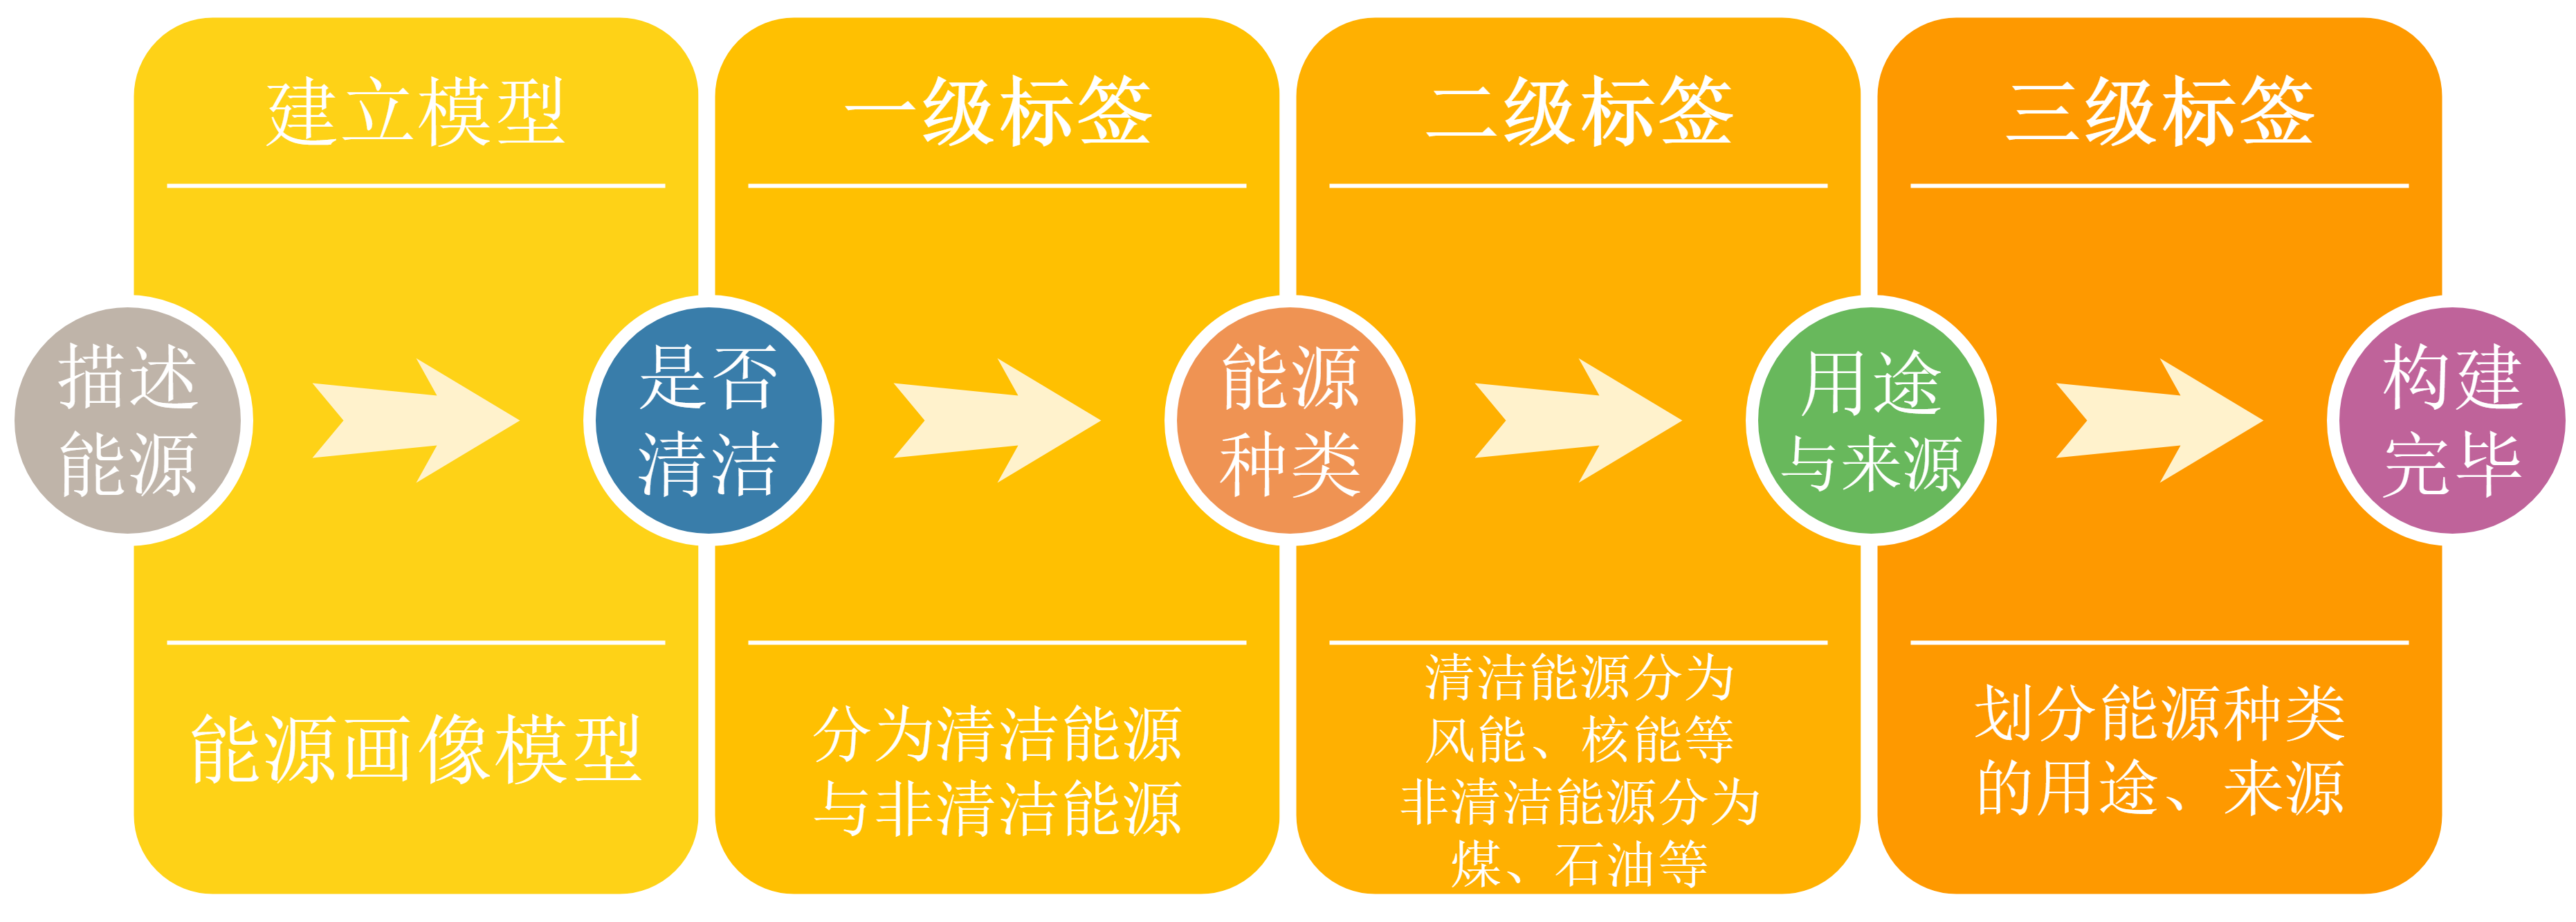
\includegraphics[width=13cm,height=4.5cm]{1.png}
	\caption{标签分级示意图} % 标题
	\label{pic1}
\end {figure}

在建立起能源画像之后,本问计算了标签权重与能源得分,详细描述了各大州的能源结构与使用情况,指出各大州主要消耗的能源与需求增长率,并且分析了各大州生产清洁能源的主要来源。
\textbf{\subsubsection{Calculate Profile Weight}}

(1)对于能够过获得数据的标签,如图\ref{pic1}中的二级标签和三级标签,使用系数变异法计算其权重。系数变异法的定义为标准差$\sigma$与均值$E(x)$的比值,能够反映出能源的使用状况和稳定状况。
\begin{itemize}
	\item 为能更详细描述能源,使用变异系数法从能源生产和消耗两个角度分别计算了各大洲的权重。记能源生产的权重为$\mathcal{W}$,能源消耗的权重为$\mathcal{Y}$。
	\item 而能源的最终目的为使用,由哪个部门使用并无区别,因此假设能源的各种用途权重均相等。
\end{itemize}
由此,计算得到的四大州各个能源的消耗权重$\mathcal{W}$如表\ref{table1}所示。

\begin{table}[h]
	\centering
	\caption{能源消耗权重}
	\begin{tabular}{cccccccc}
		\toprule
		States & BMTCB & EMTCB & ESTCB & GETCB & CLTCB & NGTCB & PMTCB\\\midrule
		AZ & 0.672 & 1.41 & 0.611 & 0.14 & 0.708 & 0.4 & 0.395 \\
		CA & 0.291 & 1.464 & 0.35 & 0.751 & 0.228 & 0.148 & 0.191 \\
		NM & 0.425 & 0.749 & 0.519 & 0.679 & 0.533 & 0.151 & 0.233 \\
		TX & 0.381 & 1.885 & 0.502 & 0.711 & 0.755 & 0.126 & 0.349 \\\bottomrule
	\end{tabular}
	\label{table1}
\end{table}
生产能源的权重$\mathcal{Y}$如表\ref{table2}所示,定义在二级标签中,同一能源的权重为生产权重与消耗权重的均值。
\begin{table}[h]
	\centering
	\caption{能源生产的权重}
	\begin{tabularx}{28em}%
		{*{5}{>{\centering\arraybackslash}X}}
				\toprule
		States & HYTCB & NUETB & SOEGB & WYTCB
		\\\midrule
		AZ&0.385 & 0.326 & 0.819 & 0.1\\
		CA&0.298 & 0.824 & 0.518 & 0.616\\
		NM&0.647 & 0 & 0 & 0.525\\
		TX&0.372 & 0.367 & 0.581 & 1.305\\\bottomrule
	\end{tabularx}
	\label{table2}
\end{table}

(2)对于抽象的概念,如图\ref{pic1}中一级标签内的清洁能源与非清洁能源,使用层次分析法确定其权重。最终得到的清洁能源的权重$\eta_1=0.75$,非清洁能源的权重为$\eta_2=0.25$。

在得到各标签之间的权重之后,以权重乘以数据得到能源使用情况的得分,至此,能源画像模型构建完毕。之后根据得分情况对各州的能源画像进行分析和表述,分析能源使用情况。
\textbf{\subsubsection{Energy Evolving}}
如图\ref{pic2}所示,对消耗的总能源而言,TX和CA州的能源使用量最高,由能源消耗的权重$\mathcal{W}$可知能源消耗以电能为主,分析数据可知能源主要用于工业和商业部门。同样,TX州和CA州对清洁能源的使用比例也相对较高,而清洁能源消耗的权重可知主要来源为风电、水电和地热能。

而对于NM州而言,清洁能源的利用率也较为良好。而详细分析NM州能源生产的权重$\mathcal{Y}$可以了解到虽然对核能和太阳能的利用较为落后,但是对风电、水电能源的利用较为良好;分析$\mathcal{W}$可知,NM州清洁能源利用率低于CA,TX州的原因为对于非清洁能源煤和天然气的使用较为频繁,应增加风电、水电的投入以减少煤和天然气的使用。
\begin {figure}[h]
	\centering % 居中显示
	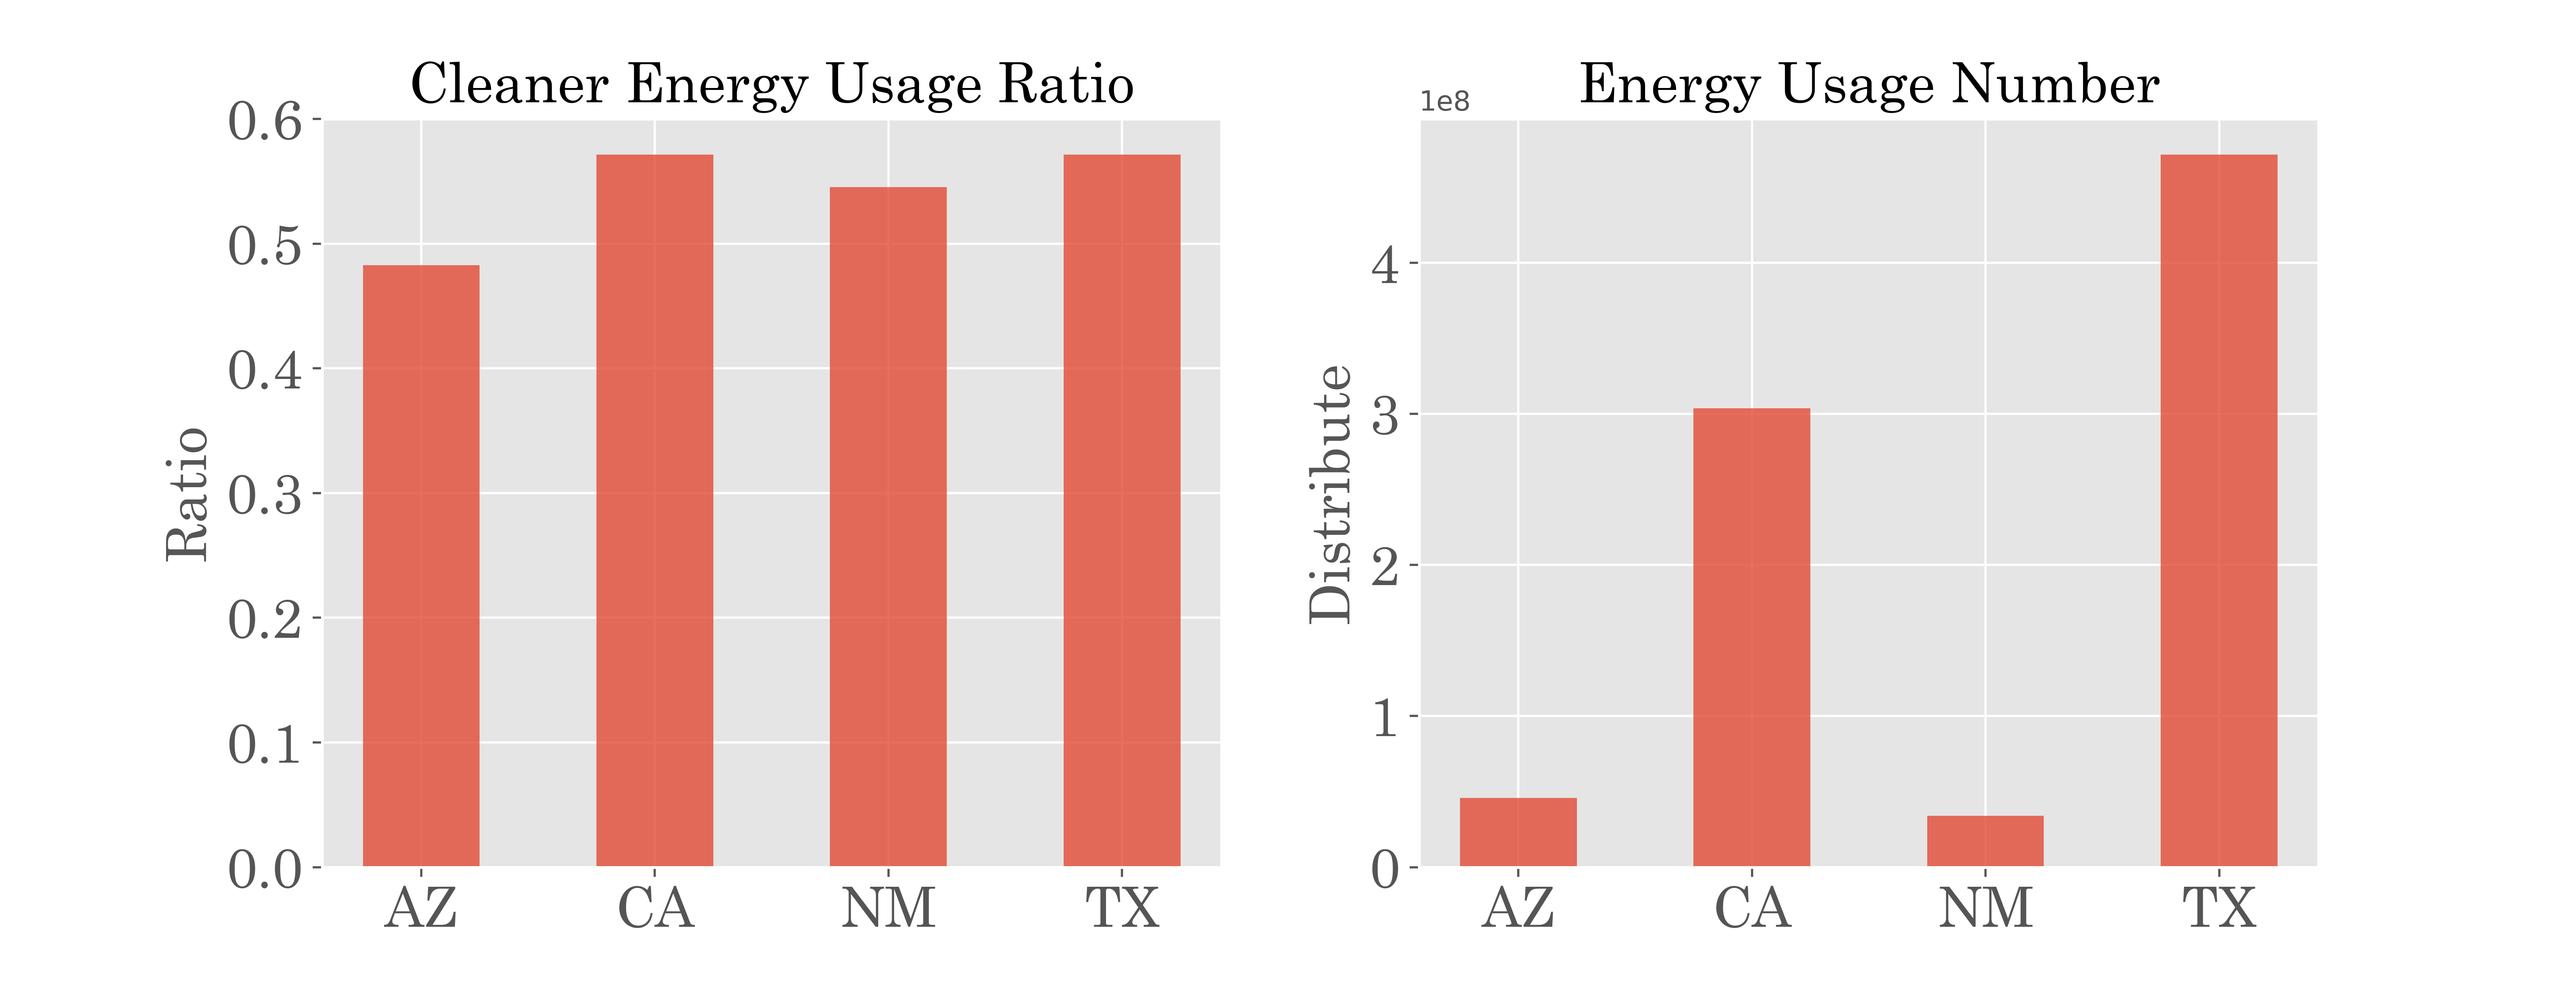
\includegraphics[width=15cm,height=5cm]{2.png}
	\caption{能源使用示意图} % 标题
	\label{pic2}
\end {figure}


\begin {figure}[h]
	\centering % 居中显示
	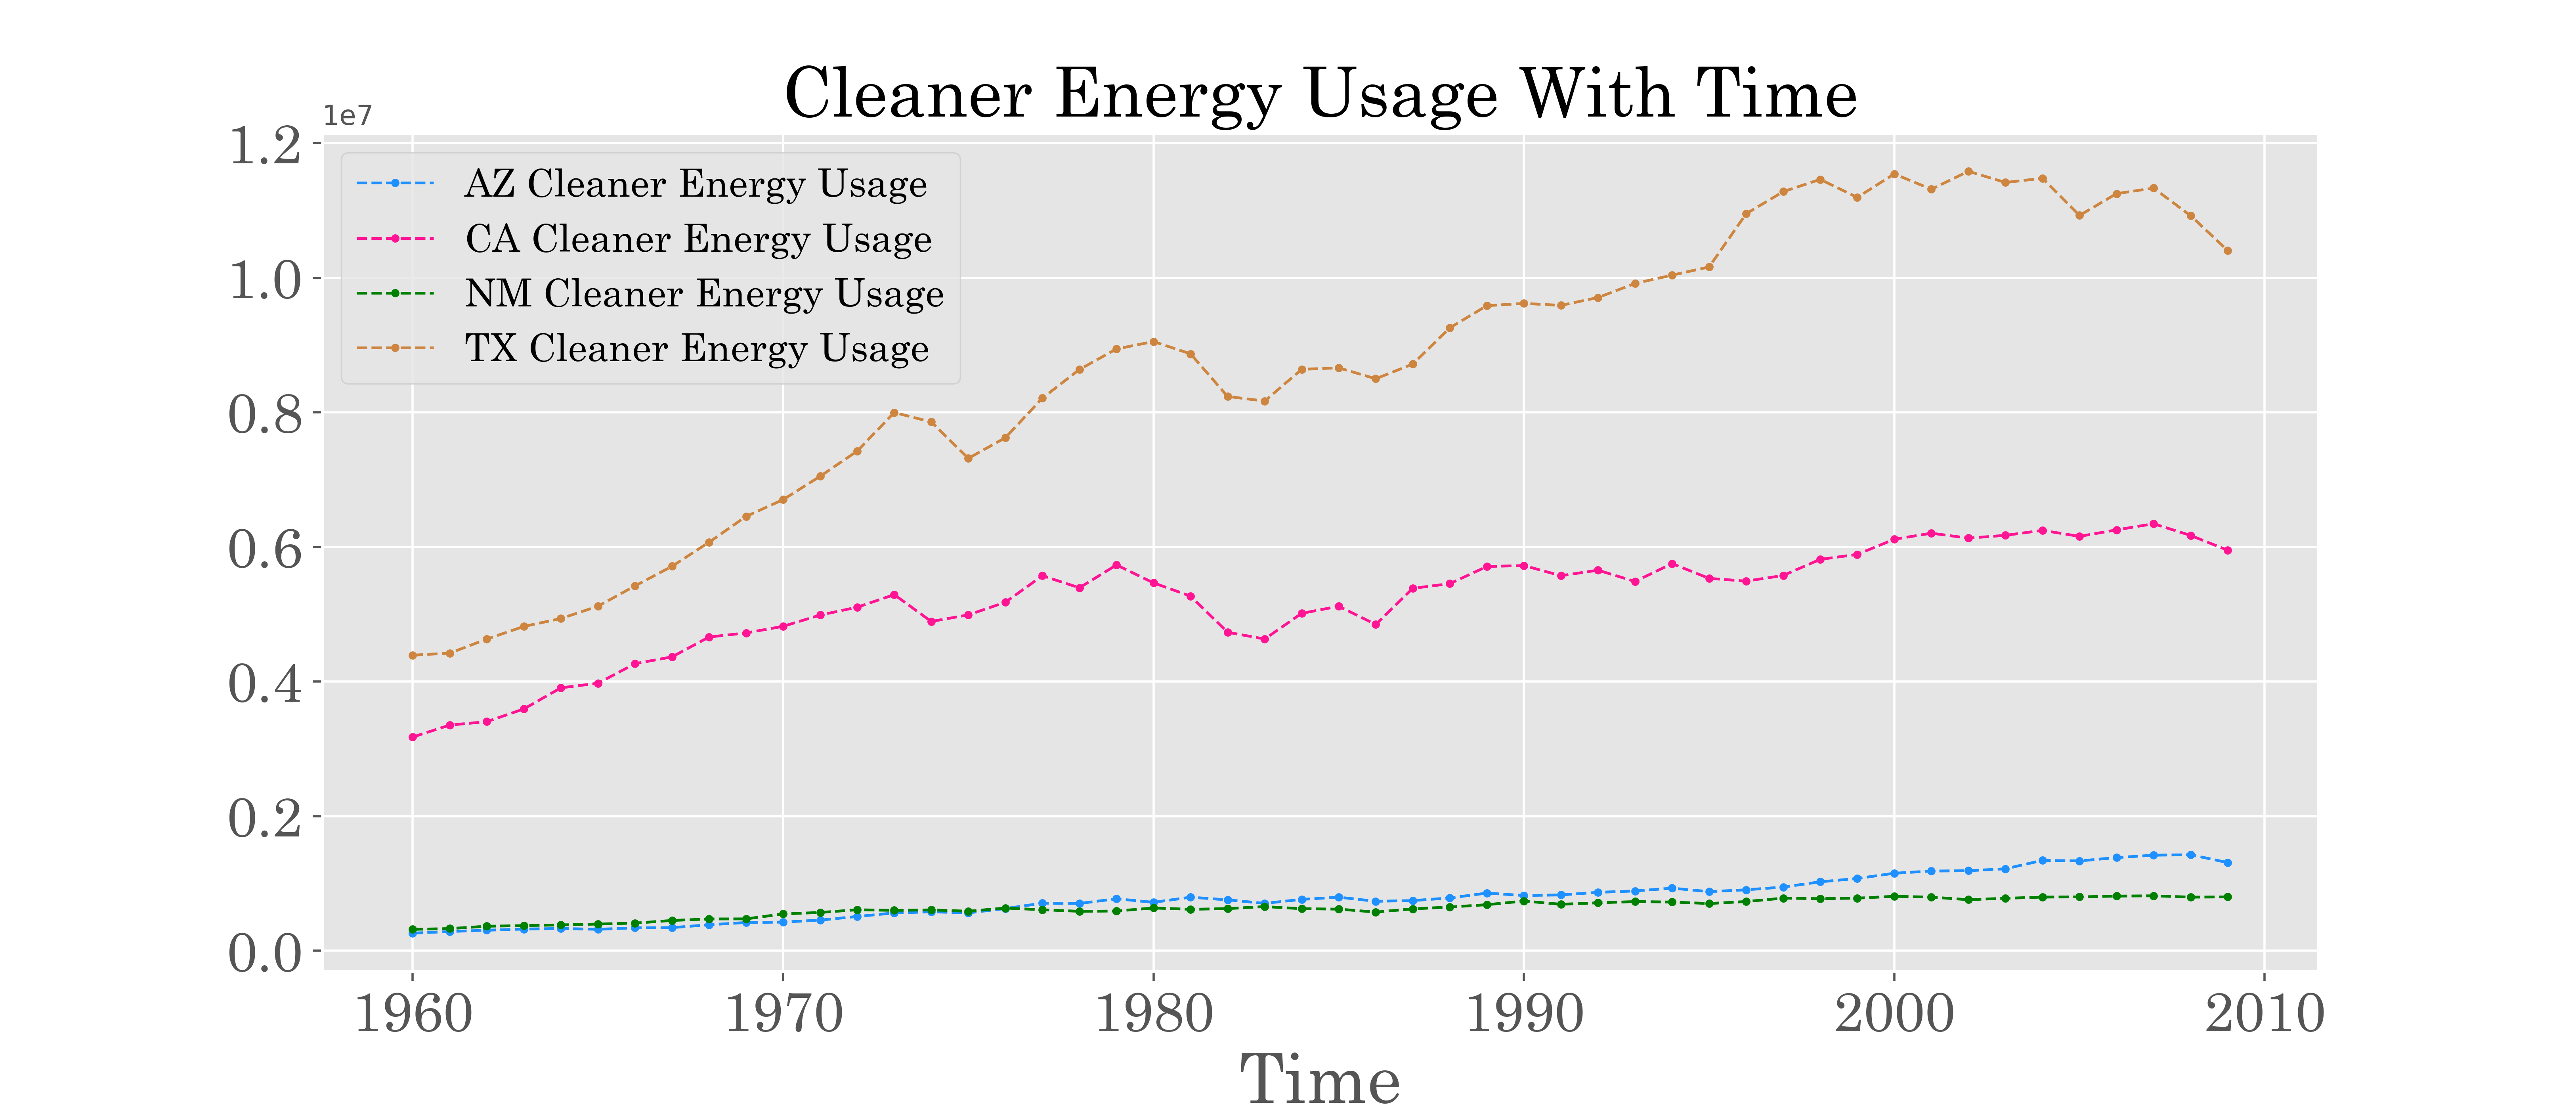
\includegraphics[width=13cm,height=6cm]{3.png}
	\caption{清洁能源使用对比图} % 标题
\label{pic3}
\end {figure}

如图\ref{pic3}所示,随着清洁环保的概念开始普及,各州的清洁能源的使用量都在上升,只是因各州情况不同而导致使用量也不相同,TX州和CA州的使用量明显高于AZ州与NM州。

为了消除能源使用基数的影响,我们定义各州在49年内清洁能源使用的增长率$\mu$:
\begin{equation}
	\mu = \mathrm{exp}(10^{-6}(\textstyle{\sum_{i=1961}^{2009}C_{i}-C_{i-1}})/49)
	\label{ratio}
\end{equation}
其中,$C_{i}$表示第$i$年的清洁能源使用量。计算得到四大州的增长率为:AZ:0.69,CA:0.76,NM:0.93,TX:0.61。表明NM州在清洁能源利用中有较大发挥空间。

\begin {figure}[h]
	\centering % 居中显示
	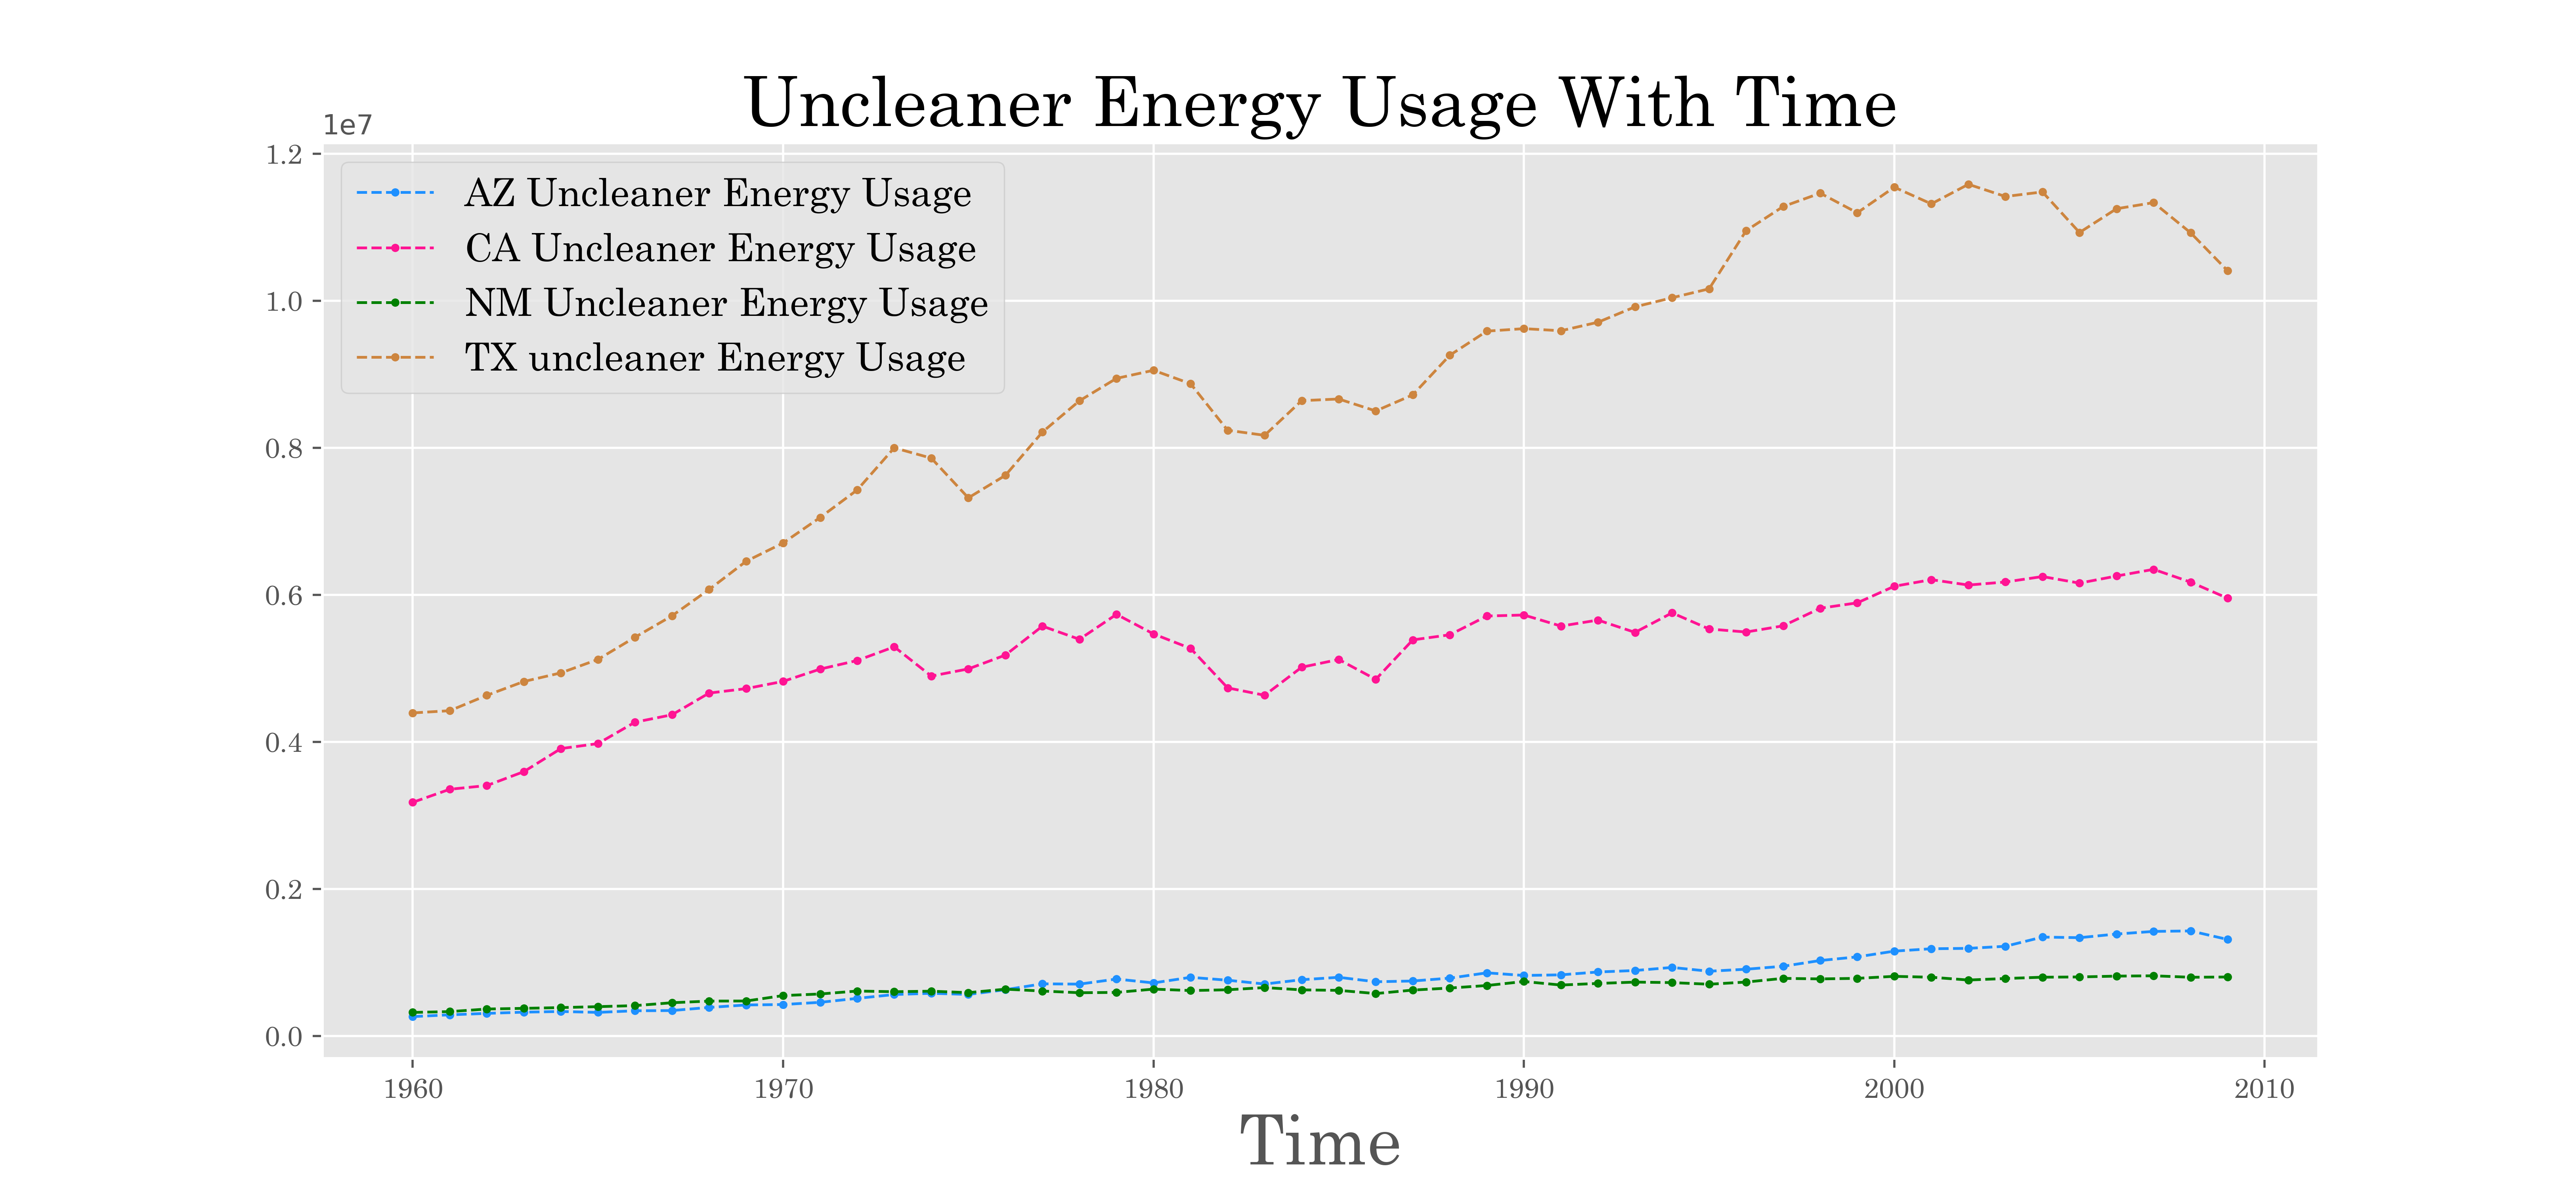
\includegraphics[width=13cm,height=6cm]{4.png}
	\caption{非清洁能源使用对比图} % 标题
	\label{pic4}
\end {figure}
如图\ref{pic4}所示,因各大州对能源总量需求不同的原因,各大州非清洁能源的消耗总量情况与清洁能源类似,CA州与TX州的消耗量明显高于AZ州与NM州。同样根据公式\ref{ratio},计算得到的四大州对非清洁能源使用的增长率,AZ:0.76,CA:0.72,NM:0.73,TX:0.64。因此可知,四大州对非清洁能源需求的增长量几乎相同。但是AZ州对非清洁能源的需求增长量最高,应增加清洁能源的使用以减少环境污染。结合$\mathcal{W}$可知,AZ州在非清洁能源的使用中,煤、石油、天然气的使用量明显高于其他州,且主要以消耗天然气为主。

而对于具体能源的描述,因电力为新时代的主要能源,本文仅以清洁能源的电能(包括风电、水电、太阳能发电求和)为例进行描述分析,其余结果见附录。
\begin {figure}[h]
	\centering % 居中显示
	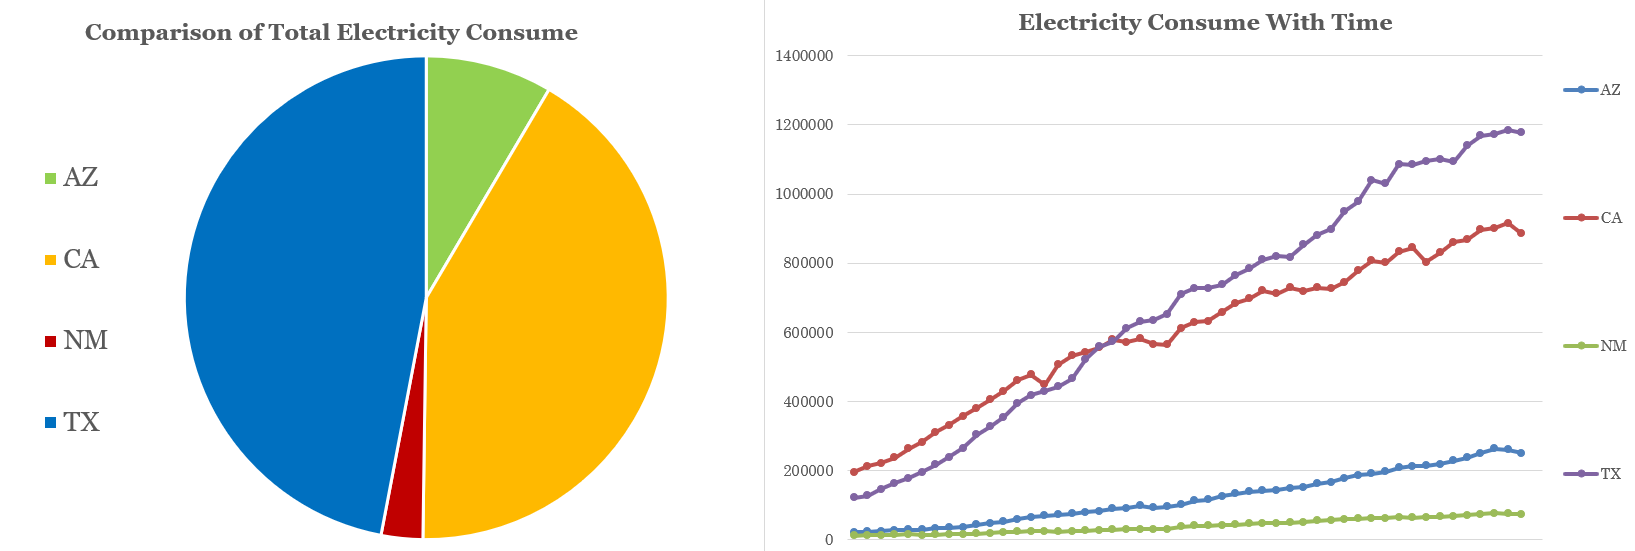
\includegraphics[width=12cm,height=4cm]{5.png}
	\caption{电力能源使用对比图} % 标题
	\label{pic5}
\end {figure}

由图\ref{pic5}所示,电力需求随时间变化而逐渐增多。TX州和CA州对于电力能源消耗多于AZ州和NM州,且结合$\mathcal{Y}$可知TX州主要以风力发电来满足电能的需求;而AZ州的风力发电较为薄弱,但以太阳能发电来满足电能的需求。同样根据公式\ref{ratio}计算电力的需求的增长率,得到以下结果:AZ:0.81,CA:0.82,NM:0.89,TX:0.61。结果显示TX州的增长率最低,NM州增长率最高结合$\mathcal{Y}$可知以水力发电为主,而CA州则以核能发电为主。
\textbf{\subsection{Model II }}
根据Model I中确定的标签权重,计算四大州清洁能源的得分情况。根据得分情况来确定衡量标准与量化差异,最后从经济与人口的角度分析产生差异的原因。

为分析四大州能源差异和相似的的原因,本文从GDP和人口数量的角度进行解释。首先,对于GDP而言,使用同公式(\ref{eq1})的方法计算各大洲的经济总量;对于人口数量而言,对人口数量进行累积求和是不合理的行为,因此选取一个区域人口最多的数量作为总人口数量。
\textbf{\subsubsection{Interpret Similarities And Differences}}
记$X$表示能源种类$x$对应的数据,$t$为时间(单位为年),以$y$表示某一能源的得分:
\begin{equation}
y=\sum_{t=1960}^{2009}\eta\cdot X_t
\end{equation}
本文从能源的生产和消耗两方面描述四大州之间的清洁能源的差异与相似点。以欧式距离量化差异的数值:
\begin{equation}
d(y_m,y_n)=\sqrt{\textstyle{\sum_{i=1}^{k}(y_m-y_n)^2}}
\label{eq1}
\end{equation}
式中以$y_m$和$y_n$表示归一化后不同大州在能源上的得分。

为了分析GDP与人口数量对清洁能源消耗造成的差异,列出清洁能源总量消耗、GDP总量(单位:百万美元)与人口数量(单位:千人),如表\ref{table3}所示。

\begin{table}[h]
	\centering
	\caption{清洁能源消耗总量}
	\begin{tabularx}{40em}%
		{*{7}{>{\centering\arraybackslash}X}}
		\toprule
		States & BMTCB & EMTCB & ESTCB & GETCB & GDP & Population
		\\\midrule
		AZ&439778.88 & 145211.63 & 3726334.64 & 1735.15 & 3941831&6587.653\\
		CA&2280690.63 & 953603.01 & 10507760.24 & 2900691.44&33604222&36887.615\\
		NM&149190.82 & 25116.71 & 1037200.37 & 7830.82&1375712&2007.315\\
		TX&1493127.04 & 554510.53 & 16969582.3 & 15110.98&18967518&24770.651 \\\bottomrule
	\end{tabularx}
	\label{table3}
\end{table}

分析差异:记不同能源的得分最高者为$y_{max}^{i}$,$i$表示能源的种类。将得分最高者评价为最佳能源“用户”。在清洁能源的使用总量中,CA州的能源评分最高,是最佳的能源使用者。而对于具体的清洁能源的最佳用户,AZ州对地热能的使用明显较差,CA州对地热能、生物质能、地热能的使用较为良好,NM州对生物质能利用明显较差,TX州对电能的使用较为广泛。

通过分析表\ref{table3}可得,表明CA州相对而言需要强大的燃料资源,政府部门应该加强粮食作物的种植和收购来增产乙醇能源,同时减少化石燃料等非清洁能源的使用;对于地热能而言,NM州和AZ州区域内阳光照射时间短,政府部门应该减少地热能的投入,转为对需求较大的能源的投入,如电力系统等,形如:结合NM州电能生产与消耗权重,NM州应加大对水电的投入,减少对核电的支出。
\textbf{\subsubsection{Analysis Influential Infactor}}
分析影响:记四大州能源总量为$G$,则$\vec{G}=(\mathrm{AZ}_{sum},\mathrm{CA}_{sum},\mathrm{NM}_{sum},\mathrm{TX}_{sum})$
$=(4313060.3,16642745.32,1219338.72,19032330.85)$。同理,能够得到GDP总量$\vec{D}$和人口总量$\vec{P}$。

计算得到$\vec{D}$和$\vec{G}$的pearsonr的相关性系数为0.84,同理得到$\vec{P}$和$\vec{G}$的pearsonr的相关性系数为0.91,均表现出较强的相关性。因此得到如下的结论:能源的消耗与区域的人口数量、经济发展程度密切相关,一个区域人口数量越多,经济越发达,则消耗的能源越多。因此,当一个区域的人口数量和经济达到一定程度时,政府部门应开始着重思考投入部分经济实力用于建设能源设备,提高能源利用率和生产率,甚至以购买的形式进口能源;此外还应该大力发展清洁能源,减少能源大量消耗带来环境污染等不良后果。
\textbf{\subsection{Model III }}
为了预测2025-2050年的能源使用情况并做出规划目标,本文从各大洲能源使用和消耗历史情况与各大洲之间的的差异两个角度出发,建立相应模型并进行求解。
\textbf{\subsubsection{Producing and Planning Goals}}
对于历史情况,设置预测步长为$s$,即使用历史$s$年的数据预测下一年的数据,而预测方的法为使用神经网络进行回归,记预测每年的得分为$T_1$。

除此之外,还需要考虑各州之间存在的差异$\vec{d}$,$\vec{d}$的各个分量为各个能源差异,则能源总消耗为$\vec{\abs{d}}$。
\begin{itemize}
	\item 考虑到现实生活中从投入能源生产、测试、运维需要较长时间,设置差异值$\vec{\abs{d}}$每$e$年更新一次$(\mathrm{参数}e=10)$。
	\item 考虑到各大州对能源的使用情况不同,NM,AZ州和TX,CA州的差异较大,而考虑较大的差异也显得不切实际。因此设TX州和CA州的差异值为$\vec{\abs{d_1}}$,设NM州和AZ州的差异值为$\vec{\abs{d_2}}$。
\end{itemize}

根据能源的历史消耗情况,假设能源消耗随时间变化服从指数分布;而能源的使用在人口、地理、气候、政治等因素影响下存在演变过程,设演变因子为$\alpha$,因此设演变过程中的差异产生的影响为$T_2$:
\begin{equation}
	T_2=\alpha\cdot \vec{\abs{d}} \cdot \sqrt[3]{t}
\end{equation}
综合考虑自身的历史演变过程和大州之间的差异,得到最终的调节方程,而求解调节方程在每年的数值即为大州的最终规划目标。

记能源使用总目标$T$,而能源的需求会随人口变化和经济发展而逐渐增长并呈现不规律的增长,因此计算出总目标$T$的取值范围,当某年的能源使用情况取值属于此区间时,认为该能源的使用情况达到了目标。规定$T$的取值范围是:$T\in[T_1, T_1+T_2]$。

\begin {figure}[h]
	\centering % 居中显示
	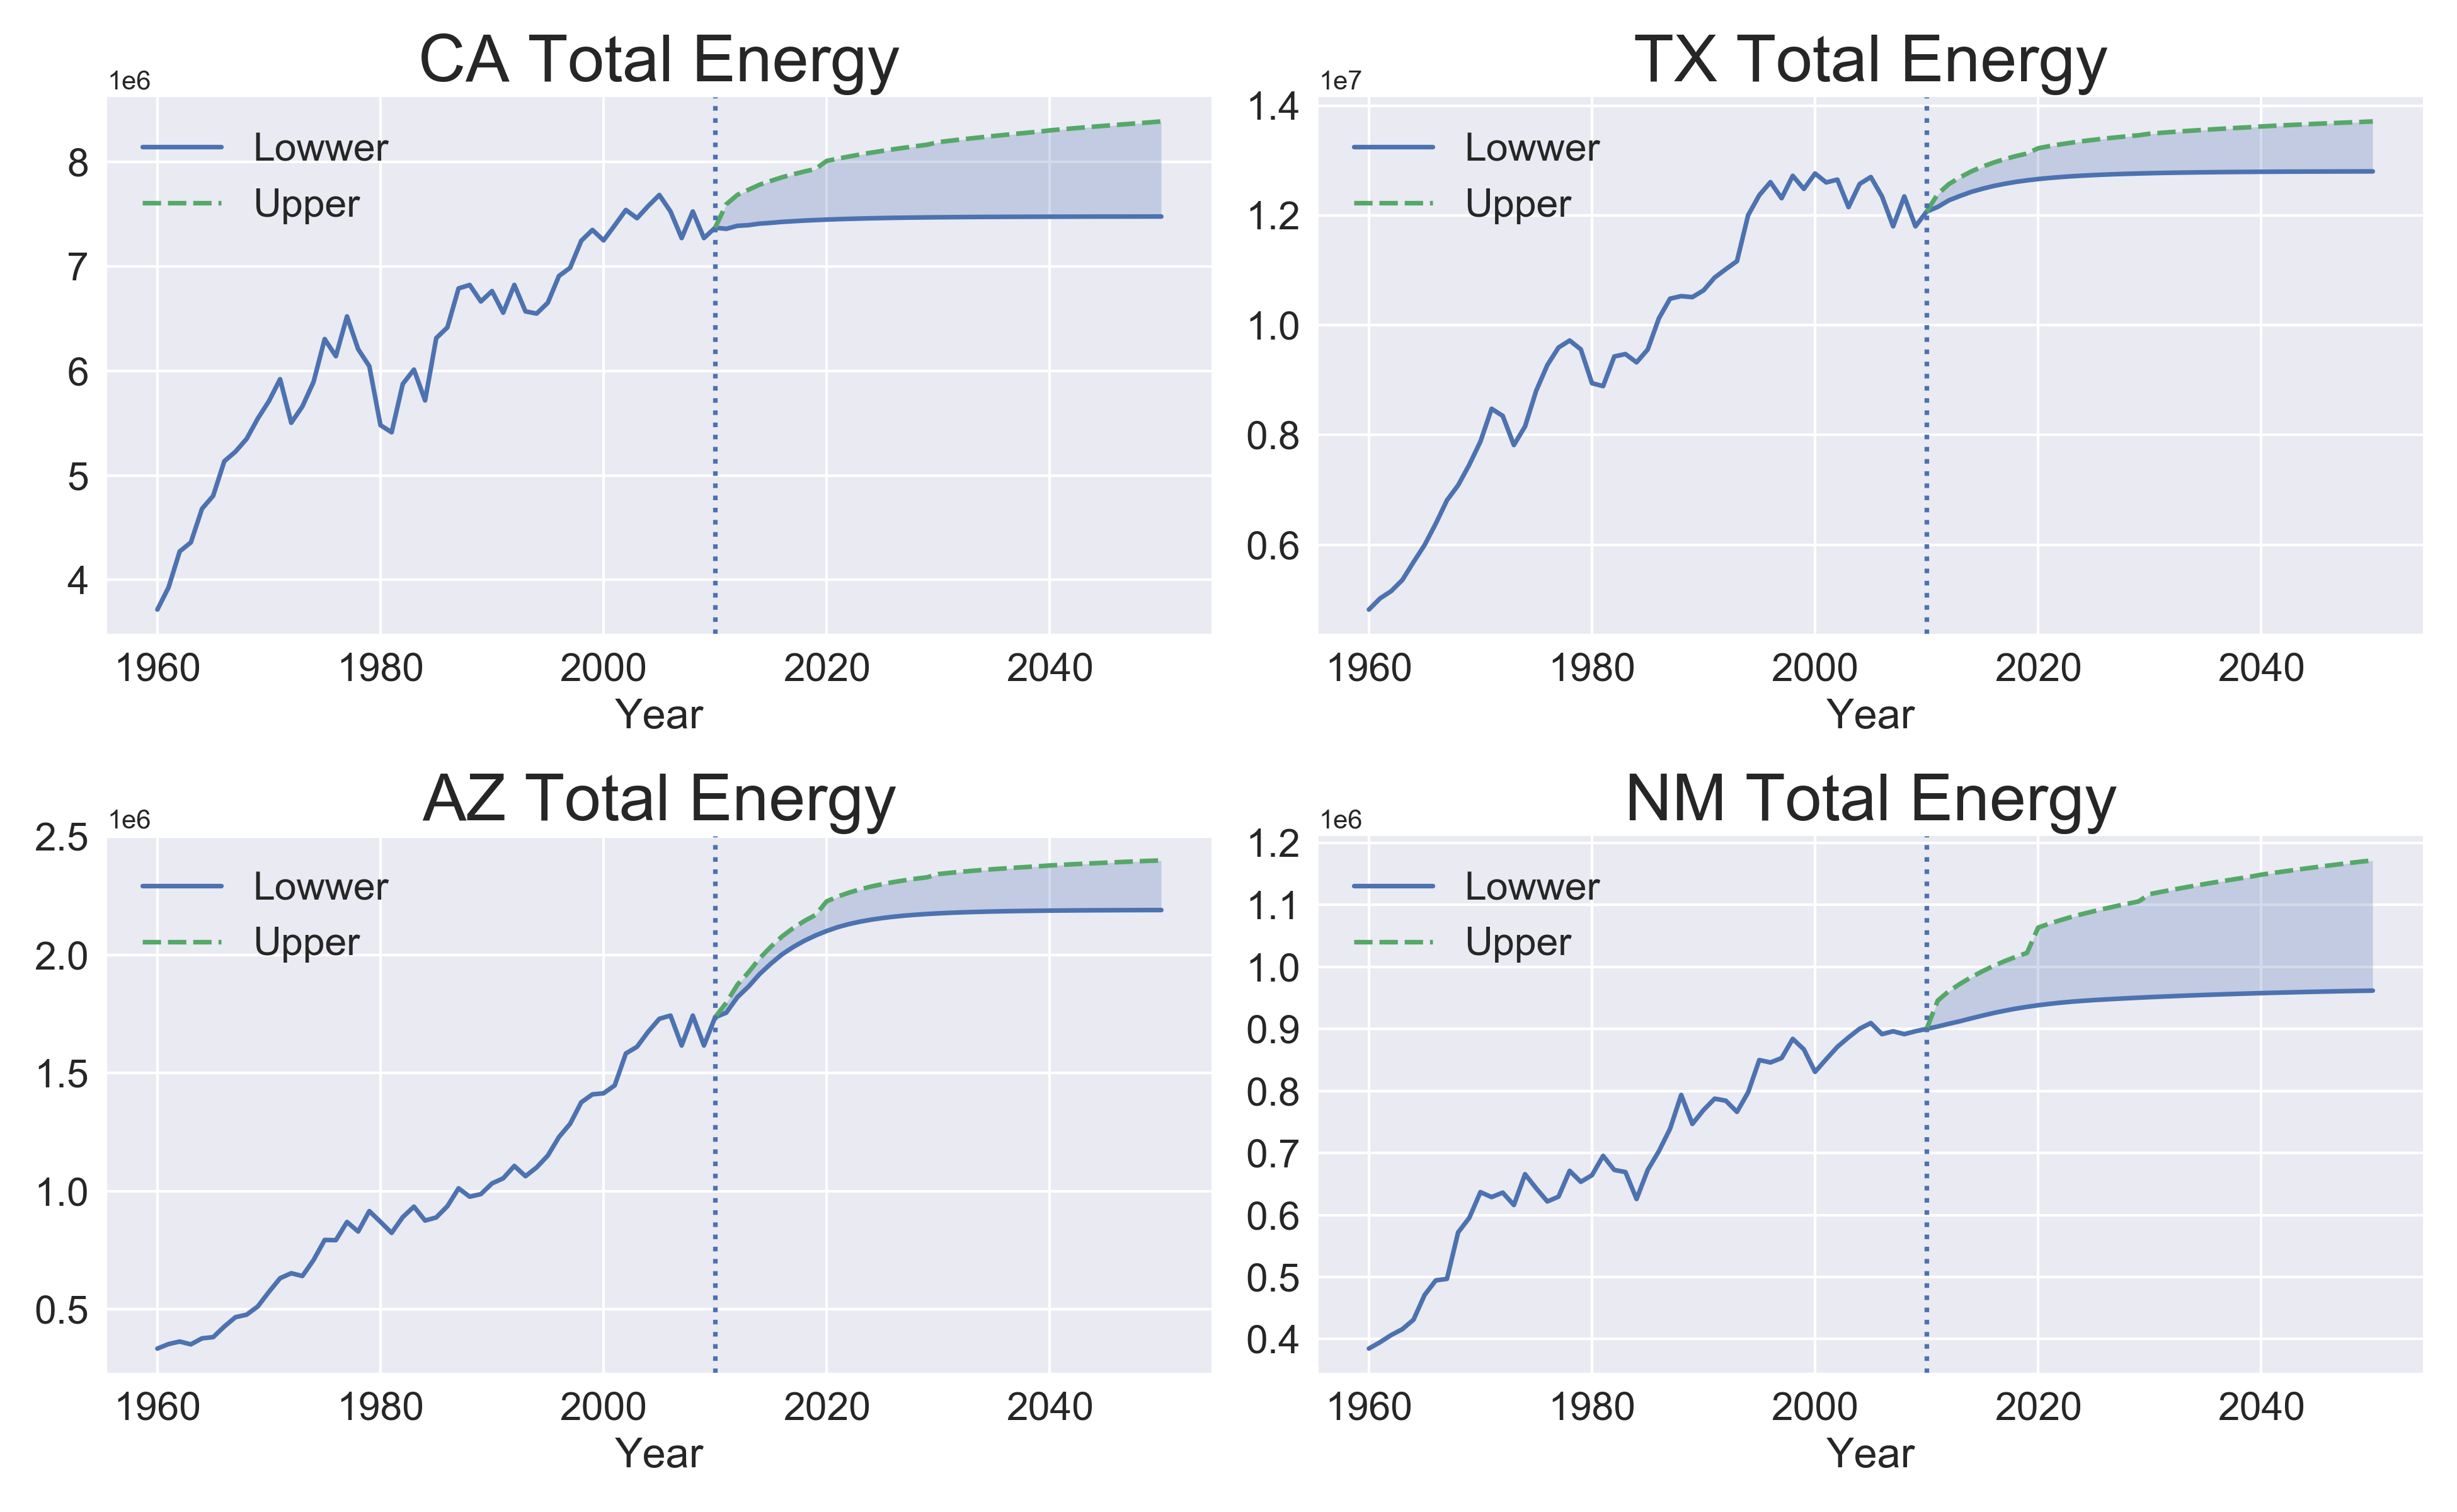
\includegraphics[width=14cm,height=8cm]{6.png}
	\caption{未来25年能源消耗目标} % 标题
	\label{pic6}
\end {figure}

得到的结果如图\ref{pic6}所示,因为对目标的规划过程中采取了弹性措施,目标值落在阴影部分内即认为达到了使用目标。图中显示出TX州具有较大的提升空间,和4.1.2小节得到的结论相同。
\begin {figure}[h]
	\centering % 居中显示
	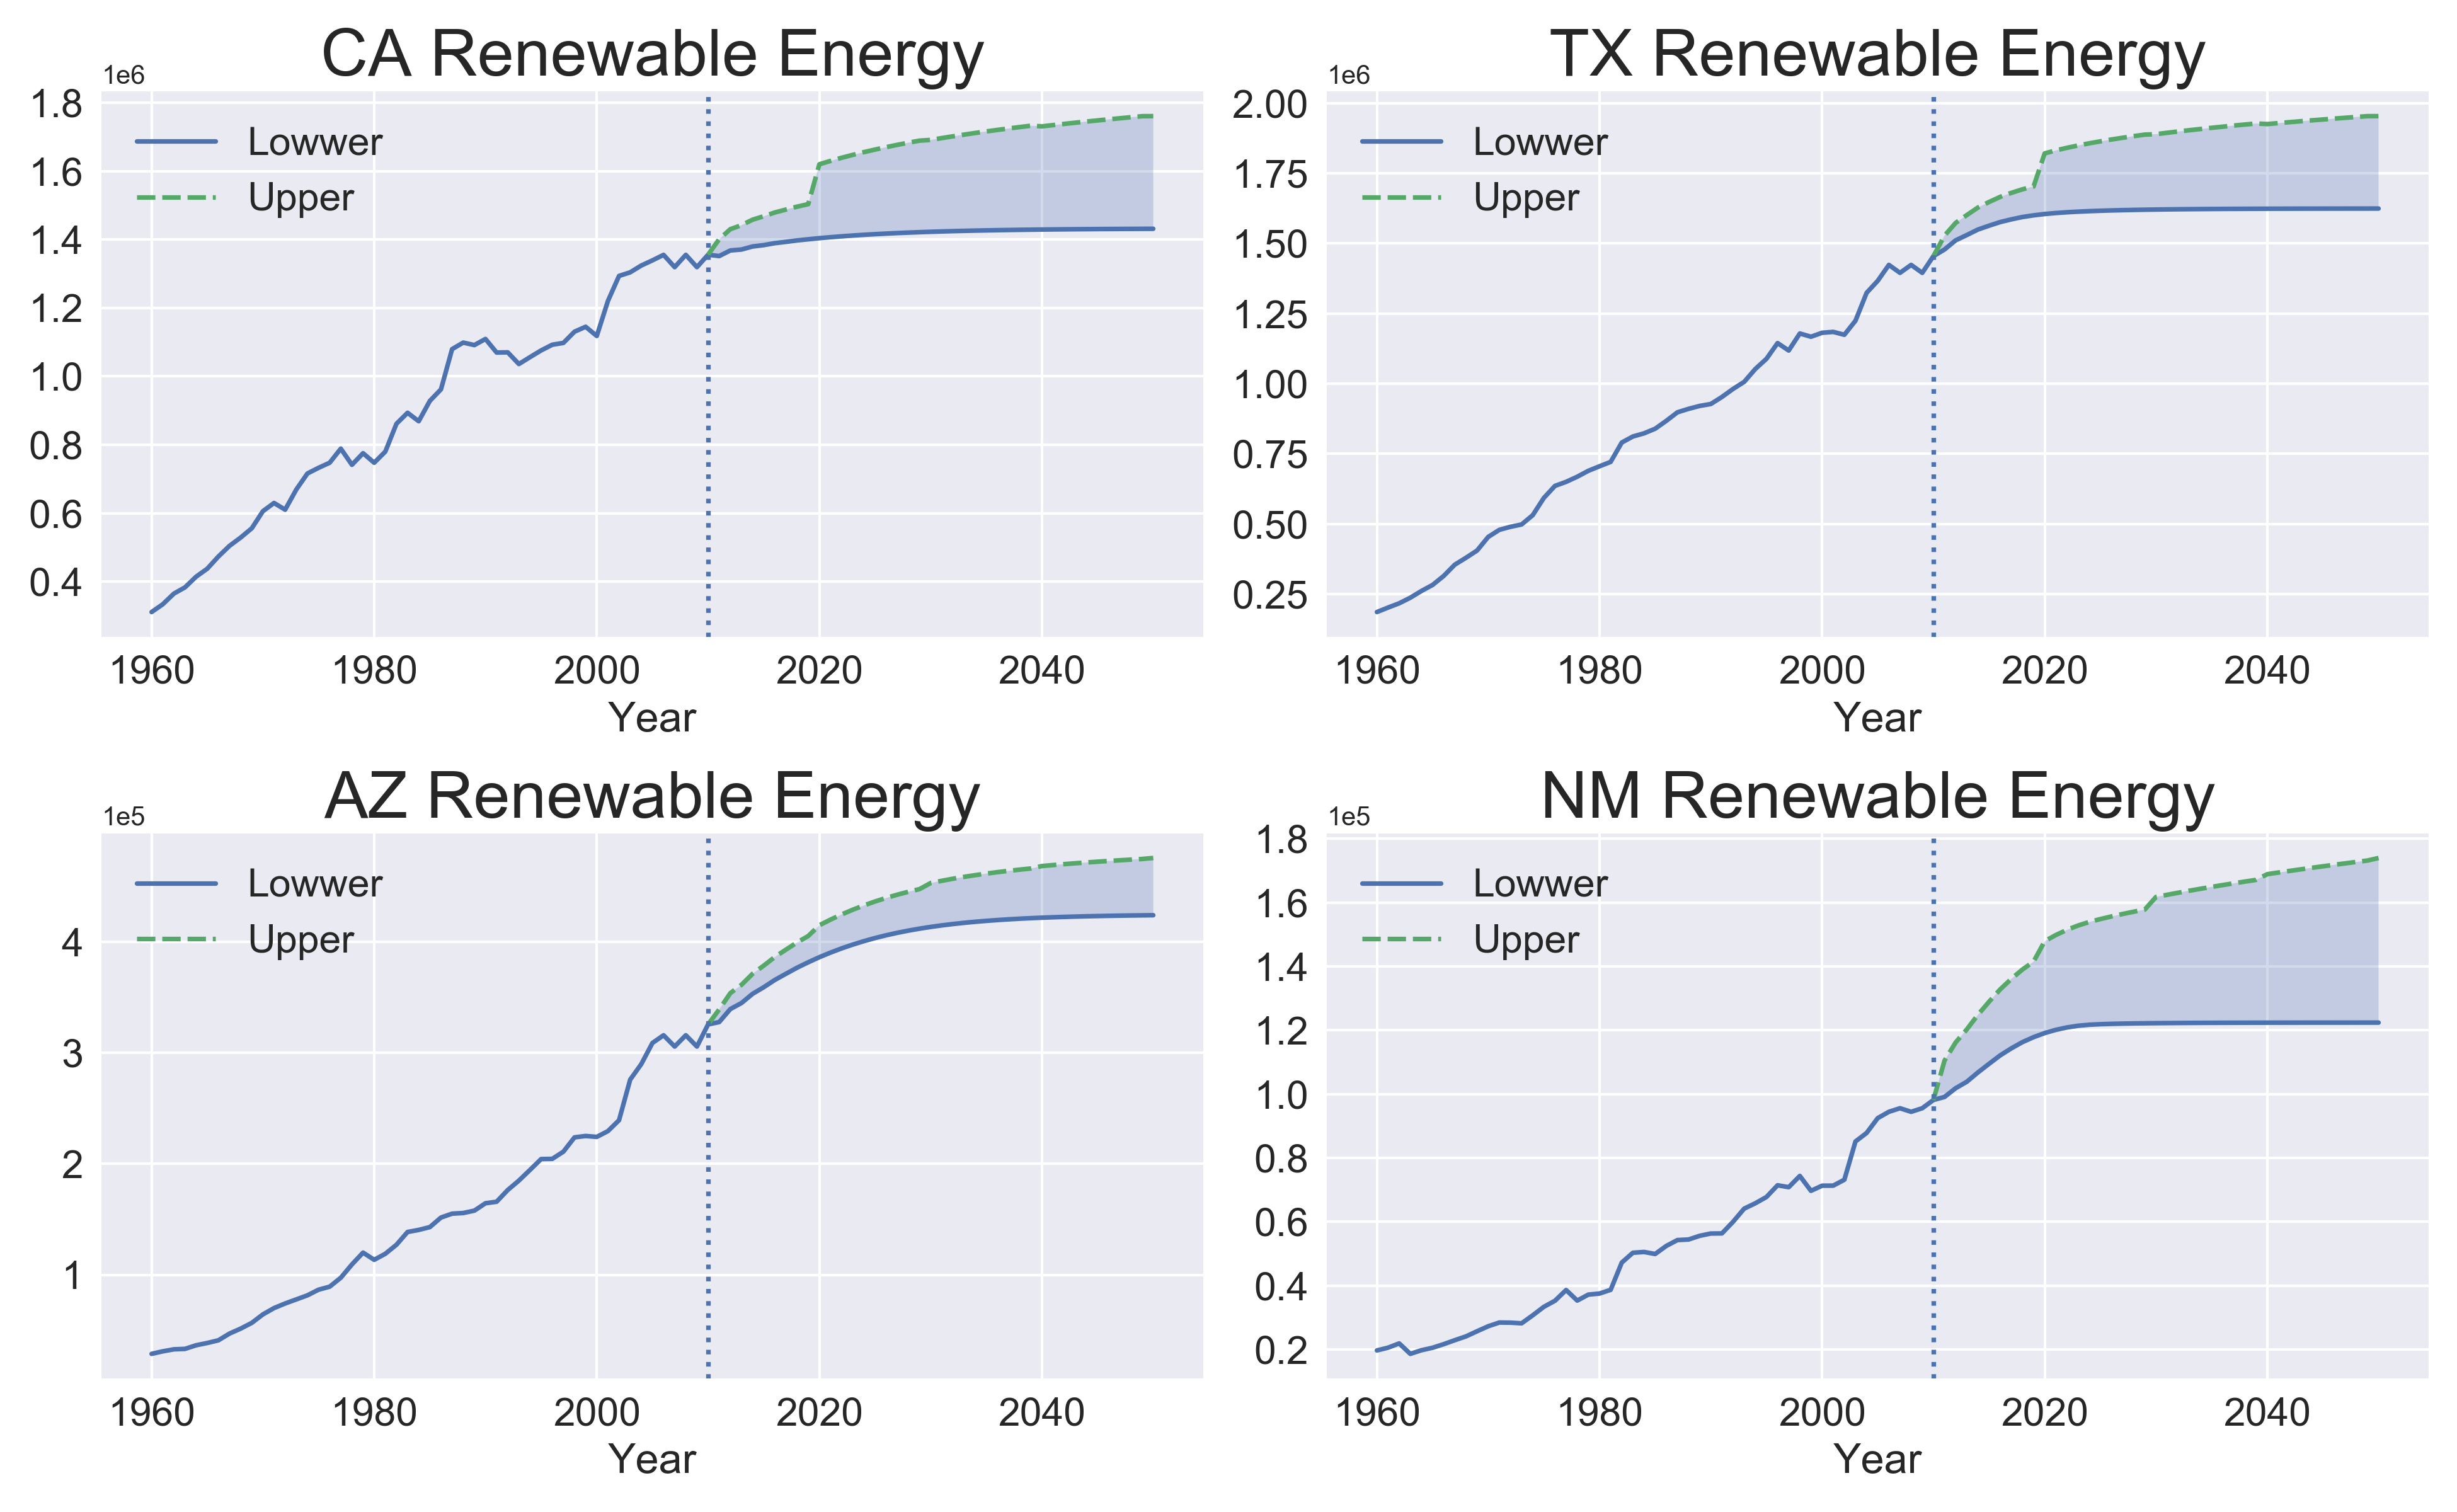
\includegraphics[width=14cm,height=8cm]{7.png}
	\caption{未来25年清洁能源消耗目标} % 标题
	\label{pic7}
\end {figure}

本文将重点分析清洁能源的使用,求解未来25年对清洁能源的消耗目标。而未来间会以消耗清洁能源为主,因此适当的对演变因子$\alpha$进行增大以扩大对清洁能源的使用,结果如图\ref{pic7}所示。

在图\ref{pic7}中,能够看出NM州需要对清洁能源的使用具有较大的上升空间,结论仍与4.1.2小节相同。结合NM州能源画像,应加大对水力发电的投入,也可以考虑对可能发电等新技术的研发,以增加清洁能源的使用量缓解能源压力。而对于其他州而言,也应保持本州的清洁能源的优势,填充不足,为日益增长的能源需求提供充足的支持,同时减少非清洁能源的使用。
\textbf{\section{Model Extension and Sensitivity Analysis}}
首先分析模型对时间、演变参数的变换后的稳定性进行了分析,在得到模型有足够的稳定性后对模型进行推广与扩展。
\textbf{\subsection{Sensitivity}}
为了检验模型的正确性,我们对模型进行灵敏性分析。未来能源消耗的目标规划对一个州的发展至关重要。因此重点对大州未来能源的发展进行灵敏性分析。

首先,我们对州未来发展的能源约束中使用的差异更新步长$e$进行检验。我们设置$e$分别取值为5,10,15,计算TX州的能源总消耗量,以分析时间因素对能源消耗总量的影响。
\begin {figure}[h]
	\centering % 居中显示
	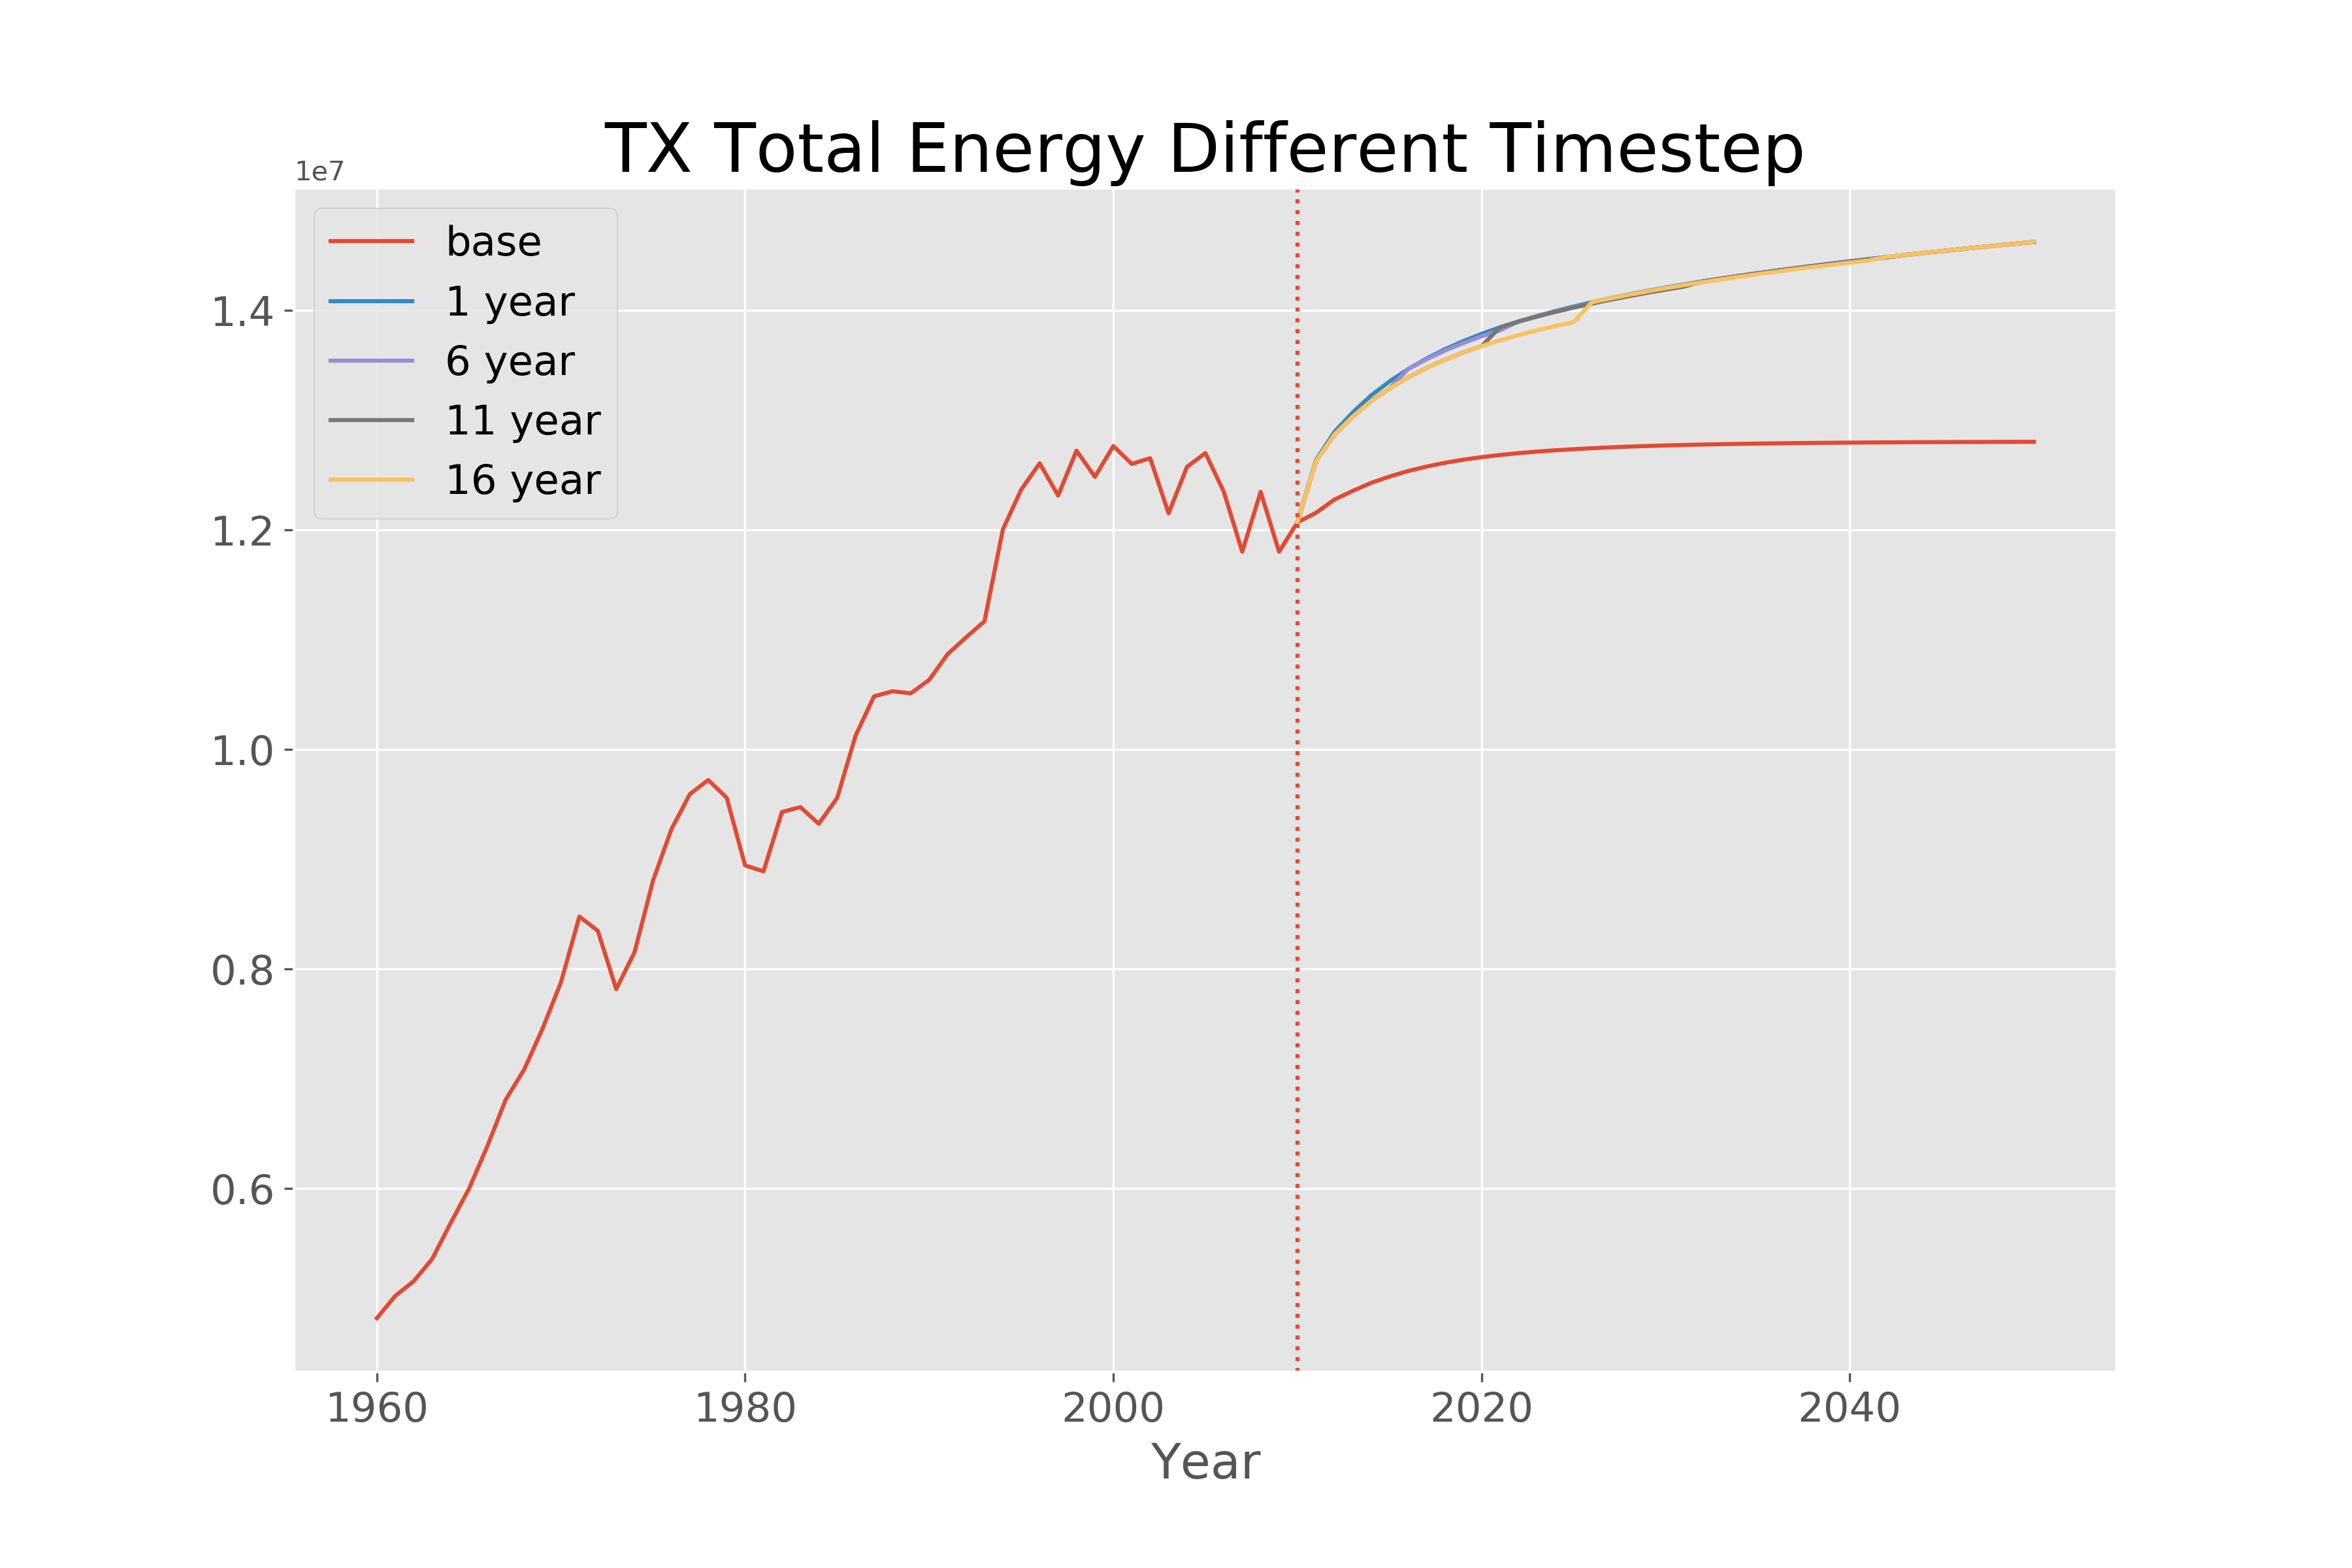
\includegraphics[width=14cm,height=8cm]{8.png}
	\caption{对$e$的灵敏性检验} % 标题
	\label{pic8}
\end {figure}

如图\ref{pic8}所示,随着步长$e$的变化,TX州在2025-2050年消耗总能源的数量并没有明显的波动。结果表明了能源使用的差异并非在十年左右的短时间内可以弥补,因此对于大州的发展计划而言,应该逐步发展基础设施和有利资源,而不应该突然的对能源投入大量成本,否则只会带来经济的负面影响,实现短时间内的超越是不切实际的行为。

其次,还应该考虑演变因子的影响,在演变因子$\alpha$取值不同的情况下对TX州2025-2050年能源总消耗量进行预测,得到的结果如图\ref{pic9}所示。

\begin {figure}[h]
	\centering % 居中显示
	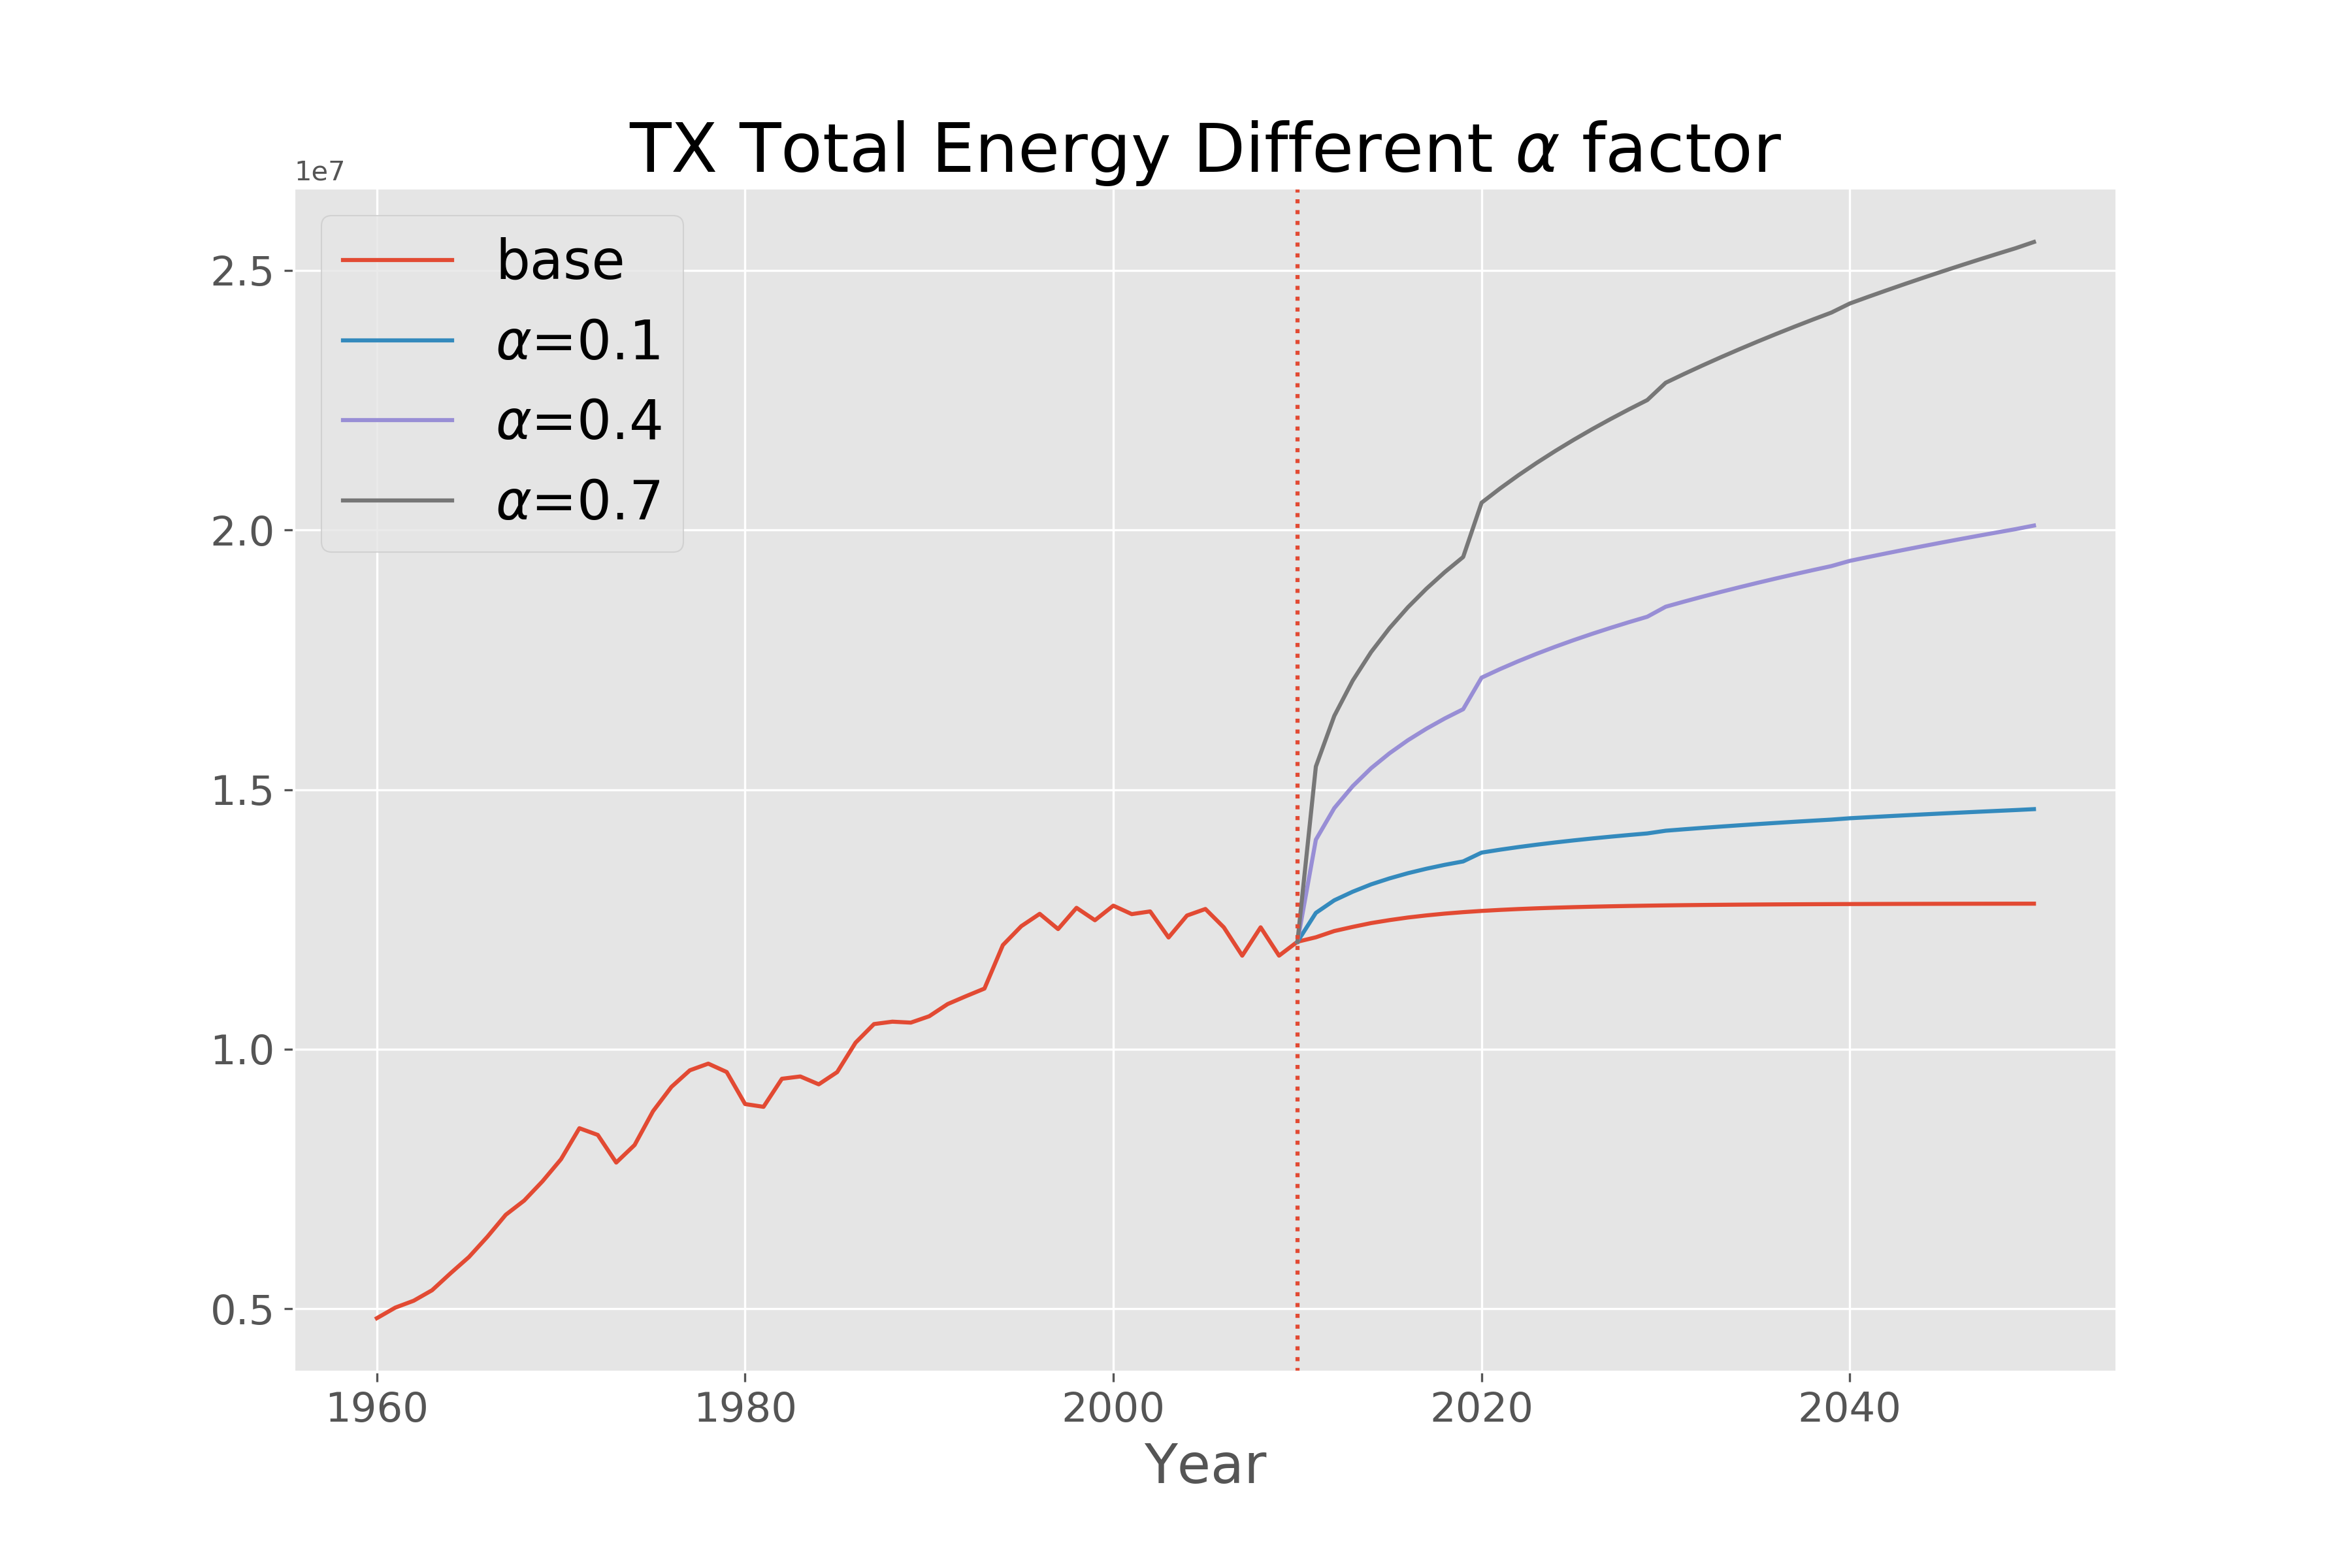
\includegraphics[width=14cm,height=8cm]{9.png}
	\caption{对差异步长$e$的灵敏性检验} % 标题
	\label{pic9}
\end {figure}

在图\ref{pic9}中,我们发现随$\alpha$的逐步增大,未来能源的消耗量也在逐步增大,因演变因子$\alpha$是综合考虑地理、气候、人口、经济等各种指标的综合因子,所以$\alpha$的取值还应考虑实际情况进行确定。总而言之,从图中能够分析出$\alpha$从正面影响着能源使用量,当确定出演变因子$\alpha$后,便可以确定出2025-2050年间的能源使用的目标情况,证明了我们模型的稳定性。
\textbf{\subsection{Model Extension}}
模型能够扩展到需要构建画像,描述结构分析异同的背景,如工业画像、经济画像和气候画像等情况。

以气候画像为例,根据一个区域的气候数据,我们能够对气候构建多级画像并计算得分,对区域的气候进行详细可量化的描述。根据得分情况分析区域之间的异同,便能够对政府部门提出合理化的建议。与此同时,还能够考虑干预政策、差异情况、历史情况对区域未来年间的气候情况进行预测,而预测数值可以代表政府部门干预气候的规划目标。
\textbf{\section{Strengths and Weaknesses}}
Based on the modeling process, we make some comments on our model as listed below.
\textbf{\subsection{Strengths}}
\begin{itemize}
	\item 构建了较为全面的能源,基于画像利用数据对画像对大州进行描述,量化的结果更容易分析异同点。
	\item 简洁明了的分析了能源使用量与人口、经济的相关性,以此对政府部门提出合理化建议。
	\item 设置弹性区间规划了未来时间内能源的使用情况,目标具有弹性限度更容易调整。
	\item 经过灵敏性分析,证明了我们的模型足够稳定。
\end{itemize}
\textbf{\subsection{Weaknesses}}
\begin{itemize}
	\item 在数据处理的过程中,删除了较多的冗余数据和缺失数据,这样处理会使得模型精度降低。如果想要改进模型,应该分析冗余数据之间的关联性。
	\item 应该搜寻更多的数据,如四大州2025-2050年中的能源基础设备情况、蕴含能源情况的数据,来提升画像的全面性与准确性。
\end{itemize}
\textbf{\section{Conclusion}}
我们建立了能源画像模型,使用不同的方法对标签确定权重,量化描述的各大州的能源分布和使用情况。并且计算了能源使用和人口、经济的相关性系数,得到了较强的相关性。之后对未来时间能源的使用情况进行了合理的预测,设置弹性区间保证结果的合理性,对应调整政策的可调度性。最终对模型的稳定性记性了检验,分别从优缺点两个方面讨论了我们的模型。
% \addcontentsline{}{}{}是添加此标题到目录
\newpage
\textbf{\section*{References}\addcontentsline{toc}{section}{References}}
\fancyhf{}
\fancyhead[R]{ }
\fancyhead[L]{ }
\bibliography{books}
\Large
\bibliographystyle{IEEEtran}
\textbf{\section*{Appendices}\addcontentsline{toc}{section}{Appendices for Code and Data}} 
\fontsize{13pt}{12.5pt}\selectfont
Here is Code we used in our model, which python is the main development language, relying on the third-party library numpy.
\vspace{7pt}
\textbf{\subsection*{Appendices A: Dynamic Program to solve Problem 1}}
\noindent{\rule{\textwidth}{0.2mm}}
\vspace{-18pt}  
\fontsize{13pt}{12.5pt}\selectfont
{
	\lstinputlisting[language=python]{data_process.py}
}
\vspace{-15pt}
\noindent{\rule{\textwidth}{0.2mm}}
\textbf{\subsection*{Appendices B: Maximum Network flow to solve Problem 2}}
\noindent{\rule{\textwidth}{0.2mm}}
\vspace{-18pt} 
\fontsize{13pt}{12.5pt}\selectfont
\vspace{-15pt}
\noindent{\rule{\textwidth}{0.2mm}}
\end{document}